\documentclass{article}
\usepackage[english]{babel}
\usepackage[margin=0.5in]{geometry}
\usepackage{longtable}
\usepackage{tabu}
\usepackage{graphicx}
\usepackage{enumitem}
\usepackage{import}
\usepackage{titlesec}
%\newcommand{\herpname}[1]{\begin{center} \Large{\textbf{#1}} \end{center}}
\newcommand{\scalegraphics}[2]{\includegraphics[scale=#2]{#1}}
\newcommand{\centeredgraphics}[2]{\begin{center} \scalegraphics{#1}{#2} \end{center}}
%\titleformat*{\section}{\Large\bfseries}

\begin{document}
\tableofcontents
\pagebreak
\section{Crocodylia --- Crocodiles and Alligators}

\subsection{Crocodylidae --- Crocodiles}
\begin{center}
\begin{longtabu} to \textwidth {| | p{3.5cm} | X | |}
	\hline
	Taxonomy/Ancestry & 
	\begin{itemize}[noitemsep]
		\item subfamilies -- crocodylinae, mekosuchinae (ex.), tomistominae
		\item \textbf{tomistominae} -- false gharial; genetic evidence suggests they are closer to the gharials so they may be reclassified into the Gavialidae family
		\item 3 extant genera; 16-17 species
		\item Ancient Greek = ``lizard of the Nile"
		\item separated from other crocodilians during Eocene epoch 55 million years ago
		\item closest living relatives are birds
	\end{itemize}
	
	\begin{center} \includegraphics[scale=0.5]{crocodylia/crocodylidae/crocodylidae.png} \end{center}
	\\
	\hline
	Size & 
	5-20 ft (1.5-6.1 m)
	
	weigh up to 2000 lb (900 kg)
	
	juveniles 20 cm (7.9 in)
	\\
	\hline
	Color & \\
	\hline
	Anatomy & 
	\begin{itemize}[noitemsep]
		\item diapsid skull
		\item dorsal scales backed by osteoderms from heavy armor plating on neck and back
		\item tail strongly muscled and flattened for swimming
		\item aquatic adaptations
			\begin{itemize}[noitemsep]
			\item nostril/ear valves
			\item nictitating membrane to cover eye
			\item glottal valve in throat
			\item able to concentrate and excrete salt; salt glands on tongue filter salt to allow for survival in saltwater environments
			\end{itemize}
		\item webbing on toes of the hind feet speeds swimming + gives advantage on dry land
		\item cerebral cortex w/ 4-chambered heart
		\item slit pupils w/ tapetum lucidum
		\item teeth are replaced throughout lifespan
		\item poikilothermic + ectothermic
		\item live 70-80 yrs
		\item distinguishing from alligators
			\begin{itemize}[noitemsep]
			\item narrower + longer heads
			\item v-shaped snouts
			\item lower teeth protrude when mouth closed
			\item large 4th tooth visible
			\item salt glands = saltwater habitat
			\item sensory pits all over body
			\item jagged fringe on hind legs + feet
			\item more aggressive + dangerous
			\end{itemize}
	\end{itemize}
	\\	
	\hline
	Dimorphism & 
	males grow larger + faster
	\\
	\hline
	Behavior & 
	\begin{itemize}[noitemsep]
		\item nocturnal hunter-scavengers
		\item often bask on shoreline
		\item aestivate during drought or arid conditions
		\item adult males bellow, growl, or hiss for dominance
		\item hatchlings grunt, squawk, communicate thru ultrasound
	\end{itemize}
	\\
	\hline
	Habitat & 
	Hill streams, large rivers, marshes, ponds, lakes, canals, reservoirs, saline habitats (i.e. mangrove creeks/saltpans)
	
	Deep water = safety + drought resistance but some species live in places where water regularly dries (Crocodylus suchus) by living in deep tunnels or caves; drought can also force species to move inland 
	\\
	\hline
	Distribution & 
	tropical + subtropical regions in Africa, Asia, Americas, Australia
	\\
	\hline
	Feeding Ecology &
	\begin{itemize}[noitemsep]
		\item opportunistic apex of the food chain
		\item young are agile + can jump to eat dragonflies, termites, spiders, other insects
		\item adolescents begin to feed on crabs, fish, frogs, reptiles, birds, + mammals
		\item scavenge for carrion
		\item teeth/jaws designed for seizing, tearing, + crushing rather than chewing
		\item some species have narrow jaws + sharp teeth to hunt fish
		\item	Sensory pores in or around mouth to help detect prey
		\item	Some species herd fish to shore w/ their bodies, often communally
		\item	Control predators of commercially important fish + help maintain cleanliness as scavengers
	\end{itemize}
	 \\
	\hline
	Reproductive Biology & 
	\begin{itemize}[noitemsep]
		\item males defend territories + compete for mates
		\item fixed breeding seasons where males mate w/ multiple females
		\item females lay eggs 40-70 days after mating; incubation period depends on nest temp (avg. 60-90 days)
			\begin{itemize}[noitemsep]
			\item higher temperatures = male, lower temperatures = female
			\item \textbf{hole-diggers} -- females dig in sand, earth, or gravel embankments above the hindwater line w/ clawed hind-limbs; eggs emerge lubricated + hatch with the wet season
			\item \textbf{mound-nesters} -- females gather vegetation, soil, or compost  and digs a hole on top to lay eggs; eggs are laid at the start of the wet season and hatch when the water is highest
			\end{itemize}
		\item females, sometimes males, guard nest during incubation
		\item young call w/ quacking grunts when ready to emerge so parents release young and carry to water
		\item young are cared for in creche formation w/ parents guarding young for 90 days
		\item adults are conditioned to respond to young distress calls
		\item mortality rate = 90\% due to predators
	\end{itemize}
	\\
	\hline
	Conservation Status &
	populations are reduced due to overhunting (for skin) and habitat loss due to human industrialization. sustainable-use programs responsible for recovery and continued survival of species like Nile, saltwater, and New Guinea crocodiles. 3 CR; 2 EN; 3 VU; 1 CD; 1 DD. 
	
	In Ancient Egypt (Sobek and Taweret), Hinduism (Varuna, Ganga, Yamuna, Goa), Aztec (Cipactli)
	 \\
	\hline 
\end{longtabu}
\end{center}
\pagebreak

\subsection{Alligatoridae --- Alligators}
\begin{center}
\begin{longtabu} to \textwidth {| | p{3.5cm} | X | |}

	\hline
	Taxonomy/Ancestry &
	subfamilies:
	\begin{itemize}[noitemsep]
		\item \textbf{alligatorinae} -- true alligators; only 1 of 10 genera currently extant; represented today by \emph{A. mississippiensis} in US and \emph{A. Sinesis} in China
		\item \textbf{caimaninae} -- caimans in C. and S. America
	\end{itemize}
	
	\begin{center} \includegraphics[scale=0.5]{crocodylia/alligatoridae/taxonomy} \end{center}
	 \\
	\hline
	Size & 
	alligator: 5-20 ft (1.5-6.1 m)
	
	caiman: average maximum weight of 6 to 40 kg (13 to 88 lb) depending on species, with the exception of the black caiman (Melanosuchus niger), which can grow more than 5 m (16 ft) in length and weigh up to 1,100 kg (2,400 lb). The average length for most of the other caiman species is about 2 to 2.5 m (6.6 to 8.2 ft) long. largest species = black caiman, smallest = Cuvier's dwarf.
	\\
	\hline
	Color &
	
	 \\
	\hline
	Anatomy &
	\begin{itemize}[noitemsep]
		\item diapsid skull
		\item armored w/ osteoderms and large scales that do not overlap
		\item forelimbs are smaller and weaker with 5 partially-webbed toes
		\item distinguishing from crocodiles:
			\begin{itemize}[noitemsep]
				\item wider, shorter heads w/ more obtuse snouts
				\item 4th enlarged underjaw tooth fits into pit in upper jaw --> no teeth visible when mouth closed
				\item no jagged fringe on hind legs + feet
				\item sensory pits appear only on snout and face, not neck and body
				\item toes of hind feet webbed not more than halfway to tips
				\item intolerant to salinity
				\item generally less aggressive and dangerous
				\item partake in foliage and fruit in addition to fish and meat
			\end{itemize}
		\item caiman characteristics:
			\begin{itemize}[noitemsep]
				\item no bony septum b/w nostrils
				\item ventral armour composed of overlapping bony scutes formed from two parts united by a suture
				\item longer, more slender, teeth than those possessed by alligators. The calcium rivets on its scales make their hides stiffer, and thus less valuable, than those of alligators and crocodiles.
			\end{itemize}
	\end{itemize}
				
	 \\
	\hline
	Dimorphism & 
	males larger and grow faster.
	
	\\
	\hline
	Behavior & 
	\begin{itemize}[noitemsep]
		\item ectotherms basking on shoreline
		\item float on surface of water
		\item become more subdued as temperatures drop but do not hibernate, making use of burrows in the winter months
		\item live in groups w/ dominance hierarchies. the highest-ranking individuals assert dominance through ritualized behaviors such as vocalizations and slapping the water with their heads.
		\item \textbf{high walk}: 4-limbed forward motion used for overland travel w/ belly up from the ground
		\item alligator holes in the wetlands increase plant diversity and provide habitats for other animals during droughts
		
	\end{itemize}
	\\
	\hline
	Habitat & 
	lakes, slow-moving streams/rivers, rivers, swamps, marshes, occasionally roadside ditches. freshwater sites w/ slow or still waters. often inhabit heavily-vegetated areas w/ muddy or murky water.
	\\
	\hline
	Distribution & 
	a New World group w/ habitats in Central-Northern S. America; parts of southern and western Central America and Mexico; SE United States; eastern China.
	\\
	\hline
	Feeding Ecology & 
	\begin{itemize}[noitemsep]
		\item opportunistic scavenger-hunters
		\item juveniles mainly eat snails and other invertebrates
		\item Typical adult diet = fish, small mammals, other reptiles (including smaller alligatorids), and birds, occasionally continuing to eat snails/invertebrates
		\item Predation typically occurs among eggs and hatchlings
		\item Racoons, coati, foxes, skunks, and other mammals, snakes, and various raptors, can raid nests or take hatchlings
		\item occasional cannibalism, but rare
		\item larger alligators help control coypu population
	\end{itemize}
	\\
	\hline
	Reproductive Biology & 
	\begin{itemize}[noitemsep]
		\item spring reproductive season
		\item courtship rituals thru loud bellowing choruses, vibrations of the male trunk
		\item use vegetables to construct nest mounds
		\item 12-60 eggs depending on species
		\item egg-laying once a year in midsummer, w/ eclosion 1-2 months afterward
		\item females respond to noises from eggs and assist offspring. offspring also use egg teeth for eclosion.
		\item females remain w/ offspring for up to 1 year.
		\item TSD is associated w/ several species, such as American alligator and common caimans. <88degF/31degC = female; >90degF/32degC = male. natural sex ratio of 5:1 female:male.
		\item Muja = oldest known in Serbia
	\end{itemize}
	\\
	\hline
	Conservation Status & 
	\begin{itemize}[noitemsep]
		\item raised commercially for their meat and skin
		\item ecotourism industry
		\item in Louisiana, heavy grazing by coypu and muskrat are damaging coastal wetlands
		\item Chinese alligator critically endangered; Louisiana and Florida zoos have some in captivity they are trying to preserve
	\end{itemize}
	\\
	\hline
\end{longtabu}
\includegraphics[scale=0.5]{crocodylia/alligatoridae/side.jpg}
\includegraphics[scale=0.5]{crocodylia/alligatoridae/top.jpg}

\end{center}

\pagebreak
\section{Testudines --- Turtles and Tortoises}

\subsection{Chelydridae - Snapping Turtle}
\begin{center}
\begin{longtabu} to \textwidth {| | p{3.5cm} | X | |}

	\hline
	Taxonomy/Ancestry &
	7 extinct, 2 extant genera.
	
	\textbf{chelydra} -- 3 species native to the Americas
	
	\textbf{macrochelys} -- much larger alligator snapping turtle, 2 species exclusively N. American forming the largest freshwater turtles in N. America. A 3rd species has been proposed, the Apalachicola.
	\begin{itemize}[noitemsep]
		\item Most closely related to Platysternidae (big-headed turtles)
		\item Sometimes considered as subfamilies within the same family, but genetic evidence supports recognition as separate families
		\item Fossil record dating from Paleocene of N. America and Oligocene of Eurasia
		\item \emph{Chelydra} is known from as far back as the Pliocene in N. America
		\item \emph{Macrochelys} is known from as far as early Miocene
	\end{itemize}
	
	\begin{center} \includegraphics[scale=0.5]{testudines/chelydridae/tax} \end{center}
	 \\
	\hline
	Size & 
	7.1-31.5 in (18-80 cm); up to 249 lb (113 kg)
	\\
	\hline
	Color &
	
	 \\
	\hline
	Anatomy &
	\begin{itemize}[noitemsep]
		\item long tail
		\item 3 rows of tubercles*
		\item hooked beak
		\item kelled*, posteriorly separated carapace
		\item reduced, cruciform*, hingeless plastron
		\item heavy claws
		\item 11 marginal scutes on each side of the carapace
		\item abdominal scutes on plastron reduced; not in contact medially
		\item carapace and plastron connected by narrow bony bridge
		\item posterior skull roof deeply emancipated
	\end{itemize}
	
	The alligator snapping turtle is characterized by a large, heavy head, and a long, thick shell with three dorsal ridges of large scales (osteoderms), giving it a primitive appearance reminiscent of some of the plated dinosaurs, most notably the ankylosaurs. They can be immediately distinguished from the common snapping turtle by the three distinct rows of spikes and raised plates on the carapace, whereas the common snapping turtle has a smoother carapace. They are a solid gray, brown, black, or olive-green in color, and often covered with algae. They have radiating yellow patterns around their eyes, serving to break up the outline of the eyes to keep the turtle camouflaged. Their eyes are also surrounded by a star-shaped arrangement of fleshy, filamentous "eyelashes".
	 \\
	\hline
	Dimorphism & 
	males larger than females
	\\
	\hline
	Behavior & 
	\begin{itemize}[noitemsep]
		\item vicious temperament; since they are on top of the food chain, they have little fear
		\item snapping jaws used against prey and predators
		\item highly aquatic but leave water to nest or travel over land to reach new habitats or lay eggs
		\item diurnal, but nocturnal activity rare in northern populations
		\item most hibernate, but many individuals are capable of going w/o hibernation and remaining active beneath ice. Hibernating snapping turtles do not breathe for, in the northern part of their range, more than six months since ice covers their hibernating site. These turtles can get oxygen by pushing their head out of the mud and allowing gas exchange to take place through the membranes of their mouth and throat. This is known as extrapulmonary respiration. If they cannot get enough oxygen through this method they start to utilize anaerobic pathways, burning sugars and fats without the use of oxygen. The metabolic by-products from this process are acidic and create very undesirable side effects by spring, which are known as oxygen debt.
		\item In shallow waters, common snapping turtles may lie beneath a muddy bottom with only their heads exposed, stretching their long necks to the surface for an occasional breath (their nostrils are positioned on the very tip of the snout, effectively functioning as snorkels).
		\item Common snapping turtles sometimes bask---though rarely observed---by floating on the surface with only their carapaces exposed, though in the northern parts of their range, they also readily bask on fallen logs in early spring. 

	\end{itemize}
	\\
	\hline
	Habitat & 
	Common habitats are shallow ponds or streams. Some may inhabit brackish environments, such as estuaries. 
	\\
	\hline
	Distribution & 
	\textbf{common snapping turtle}: southeastern Canada, southwest to the edge of the Rocky Mountains, as far east as Nova Scotia and Florida.
	
	\textbf{alligator snapping turtle}: southeastern United States waters. They are found from the Florida Panhandle west to East Texas, north to southeastern Kansas, Missouri, southeastern Iowa, western Illinois, southern Wisconsin, southern Indiana, western Kentucky, and western Tennessee. They are found on the Missouri River at least as far north as the Gavins Point Dam, the southernmost dam on the Missouri River at Yankton, South Dakota, and are featured in the Gavins Point Dam Aquarium.
	
	Located from sea level to 2000 m elevation.
	\\
	\hline
	Feeding Ecology & 
	Snapping turtles consume both plant and animal matter, and are important aquatic scavengers, but they are also active hunters that prey on anything they can swallow, including many invertebrates, fish, frogs, reptiles (including snakes and smaller turtles), unwary birds, and small mammals. In some areas, adult snapping turtles can be incidentally detrimental to breeding waterfowl, as they will occasionally take ducklings and goslings but their effect on such prey is frequently exaggerated.
	
	Common snapping turtles have few predators when older, but eggs are subject to predation by crows, mink, skunks, foxes, and raccoons. As hatchlings and juveniles, most of the same predators will attack them as well as herons (mostly great blue herons), bitterns, hawks, owls, fishers, bullfrogs, large fish, and snakes. There are records during winter in Canada of hibernating adult common snapping turtles being ambushed and preyed on by northern river otters Other natural predators which have reportedly preyed on adults include coyotes, black bears, alligators and their larger cousins, alligator snapping turtles. Large, old male snapping turtles have very few natural threats due to their formidable size and defenses, and tend to have a very low annual mortality rate
	\\
	\hline
	Reproductive Biology & 
	 Courtship is variable and poorly developed and may include direct mounting, following of the female, face-offs/head-swaying, etc.
	 
	 This species mates from April through November, with their peak laying season in June and July. The female can hold sperm for several seasons, using it as necessary. Females travel over land to find sandy soil in which to lay their eggs, often some distance from the water. After digging a hole, the female typically deposits 25 to 80 hard-shelled, but not brittle eggs each year, guiding them into the nest with her hind feet and covering them with sand for incubation and protection. Incubation time is temperature-dependent, ranging from 9 to 18 weeks. In cooler climates, hatchlings overwinter in the nest. 
	 
	 TSD: intermediate temperatures produce male offspring, while high and low extremes produce females. clutches are so large that different areas of the nest may produce different sex ratios.
	 
	 Though their potential lifespans in the wild are unknown, alligator snapping turtles are believed to be capable of living to 200 years of age, but 80 to 120 is more likely. In captivity, they typically live between 20 and 70 years.
	\\
	\hline
	Ecological Role &
	have been seen as invasive species in Italy and Japan, as well as the Czech Republic and Germany for the alligator snapping turtle.
	\\
	\hline
	Conservation Status & 
	\textbf{common snapping turtle}: used as food w/ turtle soup. The species is currently classified as Least Concern by the IUCN, but has declined sufficiently due to pressure from collection for the pet trade and habitat degradation that Canada and several U.S. states have enacted or are proposing stricter conservation measures. In Canada, it is listed as 'Special Concern' in the Species at Risk Act in 2011 and is a target species for projects that include surveys, identification of major habitats, investigation and mitigation of threats, and education of the public including landowners. Involved bodies include governmental departments, universities, museums, and citizen science projects.

	\textbf{alligator snapping turtle}: Because of collection for the exotic pet trade, overharvesting for their meat, and habitat destruction, some states have imposed bans on collecting alligator snapping turtles from the wild. The IUCN lists it as a threatened species, and as of June 14, 2006, it was afforded some international protection by being listed as a CITES III species (which will put limits on exportation from the United States and all international trade in this species). The alligator snapping turtle is now endangered in several states, including Kentucky, Indiana, Illinois, and Missouri, where they are protected by state law. They are designated as ``in need of conservation" in Kansas.
	\\
	\hline
\end{longtabu}
\includegraphics[scale=0.25]{testudines/chelydridae/common}
\includegraphics[scale=0.25]{testudines/chelydridae/alligator}
\end{center}
\pagebreak
\subsection{Kinosternidae --- Musk and Mud Turtles}
\begin{center}
\begin{longtabu} to \textwidth {| | p{3.5cm} | X | |}
	\hline
	Taxonomy/Ancestry &
	\begin{itemize}[noitemsep]
		\item 24 species within 4 genera, but taxonomic reclassification ongoing
		\item \emph{kinosternon} --- ``mud turtles," small aquatic turtles from the Americas
		\item \emph{sternotherus} --- ``musk turtles," endemic to N. America, closely related to \emph{kinosternon}
		\item \emph{claudius} --- only extant species is narrow-bridged musk turtle found in Mexico, Guatemala, and Belize
		\item \emph{staurotypus} --- Mexican musk turtles; giant musk turtles; three-kelled musk turtles; 2 recognized species found in Mexico and Central America
	\end{itemize}
	
	\begin{center} \includegraphics[scale=0.5]{testudines/kinosternidae/tax} \end{center}
	 \\
	\hline
	Size & 
	typically small, 10-15 cm (3.9-5.9 in) in length, but \emph{staurotypus} can get much larger, up to 30 cm (12 in).
	\\
	\hline
	Color &
	may be black, green, or yellowish in color. 
	
	most species don?t have shell markings, but some have radiating black markings on each carapace scute. some species have distinctive yellow striping along head and neck.
	 \\
	\hline
	Anatomy &
	\begin{itemize}[noitemsep]
		\item tall, highly domed upper carapace w/ distinct keel down center
		\item plastron differs by species
			\begin{itemize}[noitemsep] 
				\item some species have 1 or 2 hinges reaching from left to right side of shell; other species have none. the hinges allow plastron and carapace to pull tight against each other after the turtle pulls itself into the shell.
				\item some species have plastron covering only part of lower body; others have large plastron almost entirely concealing undersides
			\end{itemize}
		\item barbles* hanging from chin
		\item glands/sacs along side produce characteristic musky substance (smells like skunk spray)
	\end{itemize}
	 \\
	\hline
	Dimorphism & 
	Males usually have thicker and longer tails tipped w/ a spine; also have 2 rough, scaly patches on each leg. females are typically larger than males.
	\\
	\hline
	Behavior & 
	\begin{itemize}[noitemsep]
		\item aquatic for majority of lifespan
		\item slow swimmers
		\item travel to land for nesting or to feed during rainy season
		\item some diurnal, others nocturnal
		\item hibernation/estivation:
			\begin{itemize}[noitemsep]
				\item yellow mud turtle holds record for amt of time spent hibernating/estivating: inactive from winter to spring, summer to fall, only awakening when spring rains flood ground
				\item warm, wet climates --> active all year
				\item cold winters and deserts w/ long stretches of dry weather --> active only a few months a year and spend the rest underground waiting for better conditions
			\end{itemize}
		\end{itemize}
				
	\\
	\hline
	Habitat & 
	freshwater species living in still or slow-moving waters. prefer year-round bodies such as lakes or ponds. a few reside in shallow, seasonal ponds which have water only during a few months of the year, typically spring.
	\\
	\hline
	Distribution & 
	native to Americas
	\\
	\hline
	Feeding Ecology & 
	carnivorous turtles eating snails, clams, insects, worms, leeches, and sometimes freshly killed fishes they find. those w/ large heads typically prefer snails and clams which they can easily open w/ their jaws. in seasonal ponds, they may eat a large amount of seeds.
	\\
	\hline
	Reproductive Biology & 
	\begin{itemize}[noitemsep]
		\item no courtship rituals; mating takes place in water
		\item females go onto land to nest. they may either bury eggs in a hole they dig or simply lay eggs on surface leaves.
		\item lay 3-6 hard-shelled eggs during late spring and early summer
		\item up to 6 clutches per year
		\item oblong eggs range from 0.9-1.7 in (2.3-4.3 cm) long and from 0.6-1.0 in (1.5-2.5 cm) wide
		\item hatch 75 days to a year after being laid
		\item TSD: medium temperatures produce male offspring; females are produced by extremes
		\item post-eclosion, some species winter in subterranean nest and truly emerge in spring
		\item the yellow musk turtle is the only turtle species known to exhibit parental care. suggested to sometimes stay w/ nest and urinate on eggs long after laying to keep them moist or protect them from predators.
	\end{itemize}
	\\
	\hline
	Ecological Role &
	
	\\
	\hline
	Conservation Status & 
	4 VU; US Fish and Wildlife lists flatted musk turtle as Threatened. However, most species are quite common in their own habitats.
	\\
	\hline
\end{longtabu}
\includegraphics[scale=0.25]{testudines/kinosternidae/kino1}
\includegraphics[scale=0.5]{testudines/kinosternidae/kino2}
\end{center}

\pagebreak
\subsection{Emydidae --- Box, Pond, and Marsh Turtles}
\begin{center}
\begin{longtabu} to \textwidth {| | p{3.5cm} | X | |}
	\hline
	Taxonomy/Ancestry &
	the largest and most diverse turtle family, w/ about 50 species in 10 genera. previously, several species of Asian box turtles were classified as Emydidae but now they have been moved to another family. it contains 2 subfamilies: Emydinae and Deirochelyinae.
	
	the oldest fossils are known from Upper Cretaceous and Paleocene of N. America. in modern times, closest relatives = Geoemydidae and Testudinidae (tortoises). as recognized today, Emydidae family includes primarily New World species.
	
	\begin{center} \includegraphics[scale=0.5]{testudines/emydidae/tax} \end{center}
	 \\
	\hline
	Size & 
	10-24 in (25-60 cm)
	\\
	\hline
	Color &
	
	 \\
	\hline
	Anatomy &
	\begin{itemize}[noitemsep]
		\item most diverse turtles in appearance
		\item the carapace typically takes the form of a low arch, but is domed in some
		\item some have keels* in the form of 1-2 ridges running from the front to the back
		\item a prominent bridge often connects the carapace to the plastron
		\item typically 8 pleugrals, 5 vertebrals, and 24 marginals on carapace
		\item 12 scutes on the plastron
		\item seam b/w posterior marginal scutes and last vertebral overlap pygal bone
		\item some members have moveable hinge separating pectoral and abdominal segments
		\item small skulls
		\item toe webbing
	\end{itemize}
	 \\
	\hline
	Dimorphism & 
	Males generally smaller than females in aquatic emydids, but this may be reversed among semiaquatic and terrestrial species.
	\\
	\hline
	Behavior & 
	\begin{itemize}[noitemsep]
		\item well-developed basking habit
		\item some active year-round; others seasonally inactive
			\begin{itemize}[noitemsep]
				\item in temperate northern species, hibernacula are generally located in well-oxygenated areas of water, but painted and Blanding's turtles are tolerant of hypoxic conditions
				\item at least 2 aquatic species, chicken turtle (Deirochelys reticularia) and western pond turtle known to hibernate terrestrially
				\item eastern box turtle  (Terrapene carolina) burrows beneath leaf litter and hibernates in shallow soil to survive subfreezing temps
			\end{itemize}
		\item elaborate courtship
	\end{itemize}
	\\
	\hline
	Habitat & 
	\begin{itemize}[noitemsep]
		\item Found in diverse range of habitats
		\item Occur abundantly in most permanent freshwater rivers, streams, lakes, and ponds
		\item One species found only in estuaries/coastal waters
		\item May be semi-aquatic to fully terrestrial
	\end{itemize}
	\\
	\hline
	Distribution & 
	\begin{itemize}[noitemsep]
		\item Found in lowland temperate regions of N. America, S. Africa, southern Turkey, Middle East, and throughout Europe to southern Russia
		\item Formerly more widespread in Europe but Scandinavian populations extirpated during Pleistocene
	\end{itemize}
	\\
	\hline
	Feeding Ecology & 
	\begin{itemize}[noitemsep]
		\item Includes diets from strictly herbivorous to strictly carnivorous
		\item Hatchlings of many species highly carnivorous, but become omnivorous as they mature
		\item Some have diverse, generalized diets; others have highly specialized diets
		\item Map turtle (genus Graptemys) females may be develop huge heads w/ broad palates to crush large mollusks
		\item Chicken turtles and Blanding?s turtles independently evolved long neck w/ well-developed hyoid apparatus (elaborate bony structure that rapidly expands throat to suck in prey items)
		\item Hyoid apparatus commonly found in piscivorous turtle species
	\end{itemize}
	\\
	\hline
	Reproductive Biology & 
	\begin{itemize}[noitemsep]
		\item mating generally occurs in the spring, but some species may store sperm from earlier matings for many years
		\item many species display elaborate courtship utilizing thin forelimb claws which are vigorously waved at females; a unique pattern of head bobs may be exchanged
		\item the female allows the male to mate, suggesting the females choose whom to mate with
		\item elongated eggs may be flexible or brittle-shelled
		\item most exhibit TSD
	\end{itemize}
	\\
	\hline
	Ecological Role &
	
	\\
	\hline
	Conservation Status & 
	\begin{itemize}[noitemsep]
		\item 7 VU; 6 EN; 14 NT
		\item Human activities (eg pollution, habitat destruction, road mortality, and collection for pet trade) responsible for most species? decline
		\item Ex --- Diamondback terrapin (Malaclemys terrapin) once faced extinction due to overcollection for human consumption, but recovered as it fell out of favor w/ wealthy ppl
	\end{itemize}
	\\
	\hline
\end{longtabu}
\end{center}
\pagebreak
\subsubsection{Terrapene --- Box Turtles}
\begin{center}
\begin{longtabu} to \textwidth {| | p{3.5cm} | X | |}

	\hline
	Taxonomy/Ancestry &
	a member of the subfamily emydinae. 12 taxa over 4 species. Terrapene originally coined as genus separate from Emys for species w/ sternun separated into 2-3 divisions which can move independently.
	
	they appear abruptly in the fossil record in modern form, implying they are a generalist species able to survive under a wide variety of conditions. older fossils have been found in Nebraska dating back to the Miocene (15 Mya). only recognized extinct subspecies dates from Pliocene and was much larger than other species.
	
	\begin{center} \includegraphics[scale=0.25]{testudines/emydidae/terrapene/tax} \end{center}
	 \\
	\hline
	Size & 
	10-22cm (4-9 in)
	\\
	\hline
	Color &
	females usually have yellowish-brown eyes, while males typically have red or orange eyes.
	 \\
	\hline
	Anatomy &
	\begin{itemize}[noitemsep]
		\item distinguished by domed shell which is hinged at the bottom
			\begin{itemize}[noitemsep]
				\item allows animal to close shell tightly to escape predators
			\end{itemize}
		\item item avg. lifespan of 50 yrs, but many can live past 100. once maturity is reached, the chances of death do not seem to increase w/ age.
		\item age can be roughly estimated by counting growth rings on scutes, but estimates may be inaccurate b/c the plastron is worn smooth over time.
	\end{itemize}
	 \\
	\hline
	Dimorphism & 
	Males have concave area on plastron centered beneath hinge.
	\\
	\hline
	Behavior & 
	\begin{itemize}[noitemsep]
		\item defend selves from predation by hiding, closing shell, and biting, but are vulnerable to surprise attacks and persistent gnawing/pecking
		\item tend to move further into woods prior to hibernation
	\end{itemize}
	\\
	\hline
	Habitat & 
	\begin{itemize}[noitemsep]
		\item no standard habitat, but generally found in mesic woodlands
		\item \emph{T. ornata} can be found in grasslands
		\item desert box turtle can also be found in semidesert w/ rainfall predominantly in summer
		\item Coahuilan box turtles found only in region characterized by marshes, permanent presence of water, and cacti
	\end{itemize}
	\\
	\hline
	Distribution & 
	native to N. America, where the species w/ the widest range, the common box turtle, is found in the US and Mexico. the ornate box turtle is endemic to south-central and southwestern US/adjacent Mexico, the spotted box turtle is endemic to northwestern Mexico, and the Coahuilan box turtle found only in Cuatro Cienegas Basin in Coahuila, Mexico.
	\\
	\hline
	Feeding Ecology & 
	an omnivore w/ a varied diet, it eats anything it can catch. invertebrates/insects = principal component but diet also consists of vegetation. the diet can be amended w/ fruits. at times, it eats poisonous mushrooms, making its meat dangerous for humans.
	\\
	\hline
	Reproductive Biology & 
	relatively slow reproducers, they reach sexual maturity only after 4-5 yrs. females can store viable sperm in the oviducts for up to 4 yrs. they mate from may-october and lay elliptical, leathery eggs in flask-shaped holes 3-4 in deep in warm, sunny soil. they may have more than 1 clutch a yr, w/ avg. clutch size being larger in northern populations and ranging from 1-7 eggs. incubation takes 2-3 months. infant mortality is high, since the shell is weaker. infants may overwinter in the nest.
	\\
	\hline
	Ecological Role &
	
	\\
	\hline
	Conservation Status & 
	\begin{itemize}[noitemsep]
	\item 1 EN; 1 V; 1 NT; 1 DD
	\item Often taken as or bred as pets
		\begin{itemize}[noitemsep]
			\item Easily stressed and require more care than is generally thought
			\item Require outdoor enclosure and constant exposure to sun
			\item Recommended to buy captive bred to reduce pressure on wild populations
		\end{itemize}
	\item Some states prohibit collecting wild turtles or require permits to keep them
	\item State reptile of N. Carolina, Tennessee, Missouri, and Kansas
	\end{itemize}
	\\
	\hline
\end{longtabu}
\includegraphics{testudines/emydidae/terrapene/box}
\end{center}
\pagebreak
\subsubsection{Actinemys --- Western Pond Turtles}
\begin{center}
\begin{longtabu} to \textwidth {| | p{3.5cm} | X | |}

	\hline
	Taxonomy/Ancestry &
	emydinae subfamily. originally, its single species was considered to be part of \emph{Clemmys}.
	
	\begin{center} \includegraphics[scale=0.5]{testudines/emydidae/actinemys/tax} \end{center}
	 \\
	\hline
	Size & 
	up to 20 cm (8 in) in carapace length.
	\\
	\hline
	Color &
	dorsal color --- dark brown, dull olive.
	
	yellow plastron w/ dark blotches in acute center.
	 \\
	\hline
	Anatomy &
	\begin{itemize}[noitemsep]
		\item low, broad carapace which is widest behind the middle. in adults, it is smooth, containing no keels* or serrations.
		\item grow slowly in wild --- age at 1st reproduction may be 10-12 yrs 
		\item may survive $>$50 yrs in wild
	\end{itemize}
	 \\
	\hline
	Dimorphism & 
	males have light/pale-yellow throat.
	\\
	\hline
	Behavior & 
	frequently bask, and can be encouraged to bask on artificial surfaces for easier study.
	\\
	\hline
	Habitat & 
	\begin{itemize}[noitemsep]
		\item occur in both permanent and intermittent waters --- marshes, streams, rivers, ponds, lakes
		\item favor habitats w/ many emergent logs/boulders to bask
		\item bask on top of aquatic vegetation, and are consequently often overlooked in the environment
		\item terrestrial habitat also important b/c they can spend up to 200 days outside of water when aquatic habitat dries (intermittent ponds), and many overwinter outside the water
	\end{itemize}
	\\
	\hline
	Distribution & 
	originally, the western pond turtle ranged from northern Baja California, Mexico, north to Puget Sound, Washington. however, as of 2007, they are rare/absent in Puget Sound. they have a disjunct distribution in most of Northwest, isolated populations in southern Washington, and may be locally common in some streams, rivers, and ponds in southern Oregon. they also occur in Uvas Canyon area, Santa Cruz Mts, California, in Northbay, lakes such as Fountaingrove lake. they range up to 305 m (1,001 ft) in Washington, up to 915 m (3,002 ft) in Oregon.
	
	\begin{center} \includegraphics[scale=0.8]{testudines/emydidae/actinemys/range} \end{center}
	\\
	\hline
	Feeding Ecology & 
	omnivorous, they often eat:
	\begin{itemize}[noitemsep]
		\item insects, crayfish, aquatic vertebrates
		\item fish, tadpoles, frogs, carrion rarely
		\item filamentous algae, lily pads, tule, cattail roots
	\end{itemize}
	generally, they are well protected due to their shells, but are threatened by predators such as raccoons, otters, ospreys, coyotes. hatchlings may be preyed on by weasels, bullfrogs, large fish.
	\\
	\hline
	Reproductive Biology & 
	\begin{itemize}
		\item 5-13 eggs per clutch in annual or biannual egg-layings
		\item may travel some distance from water for egg-laying, as much as 0.8 km (1/2 mi) away from and up to 90 m (300 ft) above nearest source of water. however, most nests are within 90 m (300 ft) of water 
		\item the female leaves water in evening, selects nest site in open area of sand or hardpan facing southwards
		\item flask-shaped nest w/ abt 5 cm (2 in) opening; the female covers nest w/ soil/adjacent low vegetation
		\item the vast majority of hatchlings overwinter in the nest
		\item winter rains may be necessary to loosen hardpan soil where nest is
		\item young first appear in spring following egg deposition
	\end{itemize}
	\\
	\hline
	Ecological Role &
	
	\\
	\hline
	Conservation Status & 
	listed as VU due to human threat, they face extinction due to the removal of ponds, wetlands, and the contamination of water sources.
	\\
	\hline
\end{longtabu}
\includegraphics[scale=0.5]{testudines/emydidae/actinemys/1}
\includegraphics[scale=0.25]{testudines/emydidae/actinemys/3}
\end{center}
\pagebreak
\subsubsection{Malaclemys --- Diamondback Terrapins}
\begin{center}
\begin{longtabu} to \textwidth {| | p{3.5cm} | X | |}

	\hline
	Taxonomy/Ancestry &
	a member of the Deirochelyinae subfamily. a monotypic genus containing only the \emph{M. terrapin} species, w/ 7 subspecies recognized.
	
	\begin{center} \includegraphics[scale=0.5]{testudines/emydidae/malaclemys/tax} \end{center}
	 \\
	\hline
	Size & 
	males --- 13 cm (5.1) in; 300 g (11 oz). sexually mature at 2-3 yrs and 4-5 in of length
	
	females --- 19 cm (7.5 in); 300 g (11 oz). sexually mature at 6-7 yrs and 6.75 in of length
	\\
	\hline
	Color &
	named for the diamond patterned growth rings on carapace. unique patterns of wiggly black markings/spots on the body and head.
	 \\
	\hline
	Anatomy &
	\begin{itemize}[noitemsep]
		\item wedge-shaped shell wider from back than front
		\item large webbed feet
		\item species from warmer regions are larger
		\item adapted to marine environment near the shore
			\begin{itemize}[noitemsep]
				\item impermeable skin can stay in salt water for extended periods of time
				\item lachrymal salt glands
				\item can distinguish b/w drinking water of different salinities
				\item behavior to obtain freshwater --- drink freshwater surface layer on top of salt water during rainfall; raising head to catch rain drops
			\end{itemize}
	\end{itemize}
	 \\
	\hline
	Dimorphism & 
	females larger than males.
	\\
	\hline
	Behavior & 
	the behavior of \emph{Malaclemys} is mostly unknown due to their aquatic nature. it is suggested that nesting is the only activity that they perform on land. they most likely hibernate during colder months.
	\\
	\hline
	Habitat & 
	\begin{itemize}[noitemsep]
		\item coastal habitats --- estuaries, tidal creeks, salt marshes
		\item typically cordgrass marshes that flood at high tide, but also live in mangrove swamps in Florida
		\item survive in both freshwater and ocean water but prefer intermediate salinities
		\item no long-distance migrations
	\end{itemize}
	\\
	\hline
	Distribution & 
	narrow strip of coastal habitats on Atlantic and Gulf coasts of US --- Cape Cod to southern tip of Florida and around Gulf Coast to Texas
	\\
	\hline
	Feeding Ecology & 
	shrimps, clams, mussels, and other marine invertebrates, especially periwinkle snails.
	\\
	\hline
	Reproductive Biology & 
	see Emydidae entry for courtship and mating.
	
	\begin{itemize}[noitemsep]
		\item females wander considerable distances before nesting
		\item nest in sand dunes or scrub vegetation near ocean in June or July
		\item clutch sizes vary latitudinally ? 5.8 in S. Florida to 10.9 in NY
		\item after covering nest, female returns to ocean and does not come back to nest
		\item usually hatch in 60-85 days in August/September. the hatchlings, which are freeze-tolerant but have a lower salt tolerance, may overwinter in the nest.
		\item exhibit TSD --- warmer temperatures produce females, cooler temperatures produce males
	\end{itemize}
	\\
	\hline
	Ecological Role &
	at high densities, may eat enough invertebrates to significantly impact ecosystem, especially b/c periwinkles can overgraze important marsh plants
	\\
	\hline
	Conservation Status & 
	\begin{itemize}[noitemsep]
		\item Classified NT due to decreasing pop. \#s within range
		\item Limited protection on state-by-state level
		\item 1900s --- considered delicacy to eat, almost hunted to extinction
		\item Severely depleted by land development along Atlantic coast
		\item Receive wounds from propellors on motorboats
		\item Get trapped in crabbing/lobster nets
	\end{itemize}
	\\
	\hline
\end{longtabu}
\includegraphics[scale=0.075]{testudines/emydidae/malaclemys/1}
\includegraphics{testudines/emydidae/malaclemys/2}
\end{center}
\pagebreak
\subsubsection{Graptemys --- Map Turtles}
\begin{center}
\begin{longtabu} to \textwidth {| | p{3.5cm} | X | |}

	\hline
	Taxonomy/Ancestry &
	13 species. also known as ``sawback turtles." Member of subfamily Deirochelyinae.
	
	\begin{center} \includegraphics[scale=0.5]{testudines/emydidae/graptemys/tax} \end{center}
	 \\
	\hline
	Size & 
	Males: 3-7 in
	
	Females: 7-10 in
	\\
	\hline
	Color &
	the lines on the shell resemble waterways on maps. it has thicker, yellow lines on the limbs and face.
	 \\
	\hline
	Anatomy &
	resemble many other aquatic turtles, but distinguished by keel running length of center of carapace. some have spike-like juts along the keel. live 15-100 years.
	 \\
	\hline
	Dimorphism & 
	females larger than males. 
	
	males have much longer claws on the front legs.
	
	Females can be partitioned into 3 groups based on head width/amt of mollusks eaten --- Microcephalic (narrow, consume few mollusks); Mesocephalic (wider, mostly mollusks w/ softer-bodied prey); Megacephalic (widest, almost entirely mollusks) 
	\\
	\hline
	Behavior & 
	spend many hours basking. they are communal w/ other turtles --- share space and use each other for predator-watching.
	\\
	\hline
	Habitat & 
	\begin{itemize}[noitemsep]
		\item mostly aquatic, but spend some time on land
		\item live only in freshwater, like ponds/rivers, and prefer flowing water
		\item ideal environment = underwater plant matter to eat; rocks and logs to bask on
	\end{itemize}
	\\
	\hline
	Distribution & 
	found throughout eastern half of US and northwards into southern Canada
	\\
	\hline
	Feeding Ecology & 
	\begin{itemize}[noitemsep]
		\item more carnivorous than most Emydids
		\item females have wider heads --- eat mollusks, insects, crayfish
		\item males w/ smaller heads --- smaller mollusks and insects
		\item feeding is always in the water
	\end{itemize}
	\\
	\hline
	Reproductive Biology & 
	\begin{itemize}[noitemsep]
		\item breed in spring/fall
		\item mating takes place in deep waters
		\item nesting period in May-July
		\item prefer unshaded sites of sandy soil
		\item usually lay 2 or more clutches of 6-20 eggs
		\item hatch after 50-70 days in August-September
		\item may overwinter in nest
		\item TSD
			\begin{itemize}[noitemsep]
				\item $25^\circ$C = male
				\item 30-35$^\circ$C = female
			\end{itemize}
	\end{itemize}
	\\
	\hline
	Ecological Role &
	control invasive mollusks like zebra mussels and Asian clams
	\\
	\hline
	Conservation Status & 
	5 LC; 3 EN; 2 VU; 2 NT
	
	3 species bred heavily for pet trade in 1970s but slowly decreased in popularity
	\\
	\hline
\end{longtabu}
 \includegraphics[scale=0.75]{testudines/emydidae/graptemys/1} 
\includegraphics[scale=0.2]{testudines/emydidae/graptemys/2}
\end{center}
\pagebreak
\subsubsection{Trachemys --- Sliders}
\begin{center}
\begin{longtabu} to \textwidth {| | p{3.5cm} | X | |}

	\hline
	Taxonomy/Ancestry &
	subfamily Deirochelyinae. 16 species w/ 19 subspecies b/w them. named for how they ``slide" into the water if they sense danger while basking. also known as red-eared terrapins*.
	
	\begin{center} \includegraphics[scale=0.5]{testudines/emydidae/trachemys/tax} \end{center}
	 \\
	\hline
	Size & 
	carapace typically 15-20 cm (6-8 in).
	\\
	\hline
	Color &
	distinct broad stripe extending from right behind eye, slightly curving. the carapace is leaf green in the young, turning dark w/ age. light yellow plastron w/ dark irregular markings in the center of the scutes.
	 \\
	\hline
	Anatomy &
	\begin{itemize}[noitemsep]
		\item the carapace is oval and flattened, w/ a weak keel that is more pronounced in the young
		\item upper carapace contains vertebral scutes forming central elevated portion
		\item relies on middle ear covered by cartilaginous disc; no visible outer ear or external auditory canal
		\item live 20-30 years; shorter in captivity
	\end{itemize}
	 \\
	\hline
	Dimorphism & 
	females larger.
	
	males have longer claws on front feet to hold female during mating. thicker and longer tail holding dark colored, retractable penis.
	
	in the male, the cloaca is beyond the edge of the carapace, while in the female, it is at or under the rear edge of the carapace.
	
	the male's plastron is slightly concave, while the female's is completely flat.
	\\
	\hline
	Behavior & 
	\begin{itemize}[noitemsep]
		\item often seen basking in groups
		\item almost entirely aquatic but bask to maintain body temp.
		\item do not hibernate, but brumate*
			\begin{itemize}[noitemsep]
				\item occasionally rise to surface for food, drink, or air
				\item inactive in October when temp $< 10\circ$C (50$\circ$F) --- enter state of topor and do not eat or defecate, remain motionless, less breathing, may become active during warmer times in winter but return when temp drops
				\item survive anaerobically producing ATP from glycolysis w/ dropped metabolic rate
				\item do not brumate* if captive
			\end{itemize}
	\end{itemize}	
	\\
	\hline
	Habitat & 
	exclusively freshwater, they live in habitats w/ rocks or logs to bask on.
	\\
	\hline
	Distribution & 
	native to the Americas, they range from the US to northern Argentina.
	\\
	\hline
	Feeding Ecology & 
	Young pond sliders tend to be more carnivorous than adults, eating about 70\% animal matter and 30\% plant matter. Adults eat 90\% plant matter and 10\% animal matter. Foods include aquatic insects, snails, tadpoles, crawfish and other crustaceans, and fish. They also eat plants like arrowhead, water lilies, hyacinths, and duck weed. Feeding occurs under water, usually in the early morning or late afternoon.
	
	Pond slider eggs and hatchlings are preyed on by raccoons, skunks, opossums, foxes, and other predators. They are relatively safe from most predators once they reach adult size and while they are in the water. Large predatory fish seem to find the hatchlings difficult to handle and do not tend to eat them. Red-eared sliders may attempt to bite and scratch when harassed, but most pull their head and legs into their shells for protection.
	\\
	\hline
	Reproductive Biology & 
	\begin{itemize}[noitemsep]
		\item mating takes place from March-July
		\item courtship --- male swims around female and flutters claws around her head; if receptive, female swims toward male and sinks to bottom for mating
		\item courtship = 45 min, mating = 10 min
		\item on occasion male appears to be courting another male; may be sign of dominance or preclude fight
		\item post-mating, female spends extra time basking to keep eggs warm. she may change her diet.
		\item can lay 2-30 eggs, up to 5 clutches a year
		\item actual egg fertilization takes place during egg-laying --- female can lay fertile eggs in following season w/o mating
		\item during last weeks of gestation female spends time scratching at ground to find suitable place
		\item Incubation = 59-112 days
		\item hatchling breaks egg w/ egg tooth
		\item may overwinter in nest
		\item new hatchling has yolk sac attached to stomach which will be absorbed; damaging yolk sac = death $\rightarrow$ when relocating eggs, always mark top so they don't get flipped over and let sac strangle baby
	\end{itemize}
	\\
	\hline
	Ecological Role &
	Pond sliders help to control populations of the animals that they consume and affect aquatic vegetation as they graze. Young pond sliders are an important food source for large, aquatic predators.
	\\
	\hline
	Conservation Status & 
	\begin{itemize}[noitemsep]
		\item most commonly traded reptile
		\item when mature, they can bite, which results in them being dumped into the wild
		\item asymptomatic carriers of salmonella; FDA banned selling turtle eggs and turtles w/ carapace length under 4 in (10 cm)
		\item considered significant threat to native turtle species in Australia; high social/economic costs predicted
	\end{itemize}
	\\
	\hline
\end{longtabu}
\includegraphics[scale=0.25]{testudines/emydidae/trachemys/1}
\includegraphics[scale=0.75]{testudines/emydidae/trachemys/2}
\end{center}
\pagebreak
\subsubsection{Chrysemys --- Painted Turtles}
\begin{center}
\begin{longtabu} to \textwidth {| | p{3.5cm} | X | |}

	\hline
	Taxonomy/Ancestry &
	1 species, \emph{C. picta}, w/ 3 subspecies. Member of subfamily Deirochelyinae.
	
	it is commonly found in the fossil record. the oldest samples are from Nebraska 15 mya. most recent fossils are widely distributed; fossils $<$ 300,000 years old are found throughout the US and southern Canada. 
	
	\begin{center} \includegraphics[scale=0.5]{testudines/emydidae/chrysemys/tax} \end{center}
	 \\
	\hline
	Size & 
	female: 10-25 cm (4-10 in); 500 g (18 oz)
	
	male: 7-15 cm (3-6 in); 300 g (11 oz)
	\\
	\hline
	Color &
	red/yellow stripes on neck, legs, and tail.
	 \\
	\hline
	Anatomy &
	upper jaw = philtrum (shaped like inverted V) w/ downward, tooth-like projection on either side. Distinguish from red-eared slider: \emph{Chrysemys} is flatter; slider has red ``ear" marking and spotted bottom shell
	 \\
	\hline
	Dimorphism & 
	females larger than males. the female has a higher, more rounded carapace, and the male has longer foreclaws; longer, thicker tail; cloaca located farther out on tail
	\\
	\hline
	Behavior & 
	\begin{itemize}[noitemsep]
		\item emerges at sunrise to bask, then goes to water to forage; repeats cycle until night when it sinks to the bottom to sleep
		\item must maintain $17-25^\circ$C internal body temperature to be active
		\item spring --- forages at water temp $15-18^\circ$C but not if temp exceeds $30^\circ$C
		\item fall --- stops foraging when temperature is below$15-18\circ$C
		\item winter --- hibernation
			\begin{itemize}[noitemsep]
				\item in the north, they can hibernate as long as October-March
				\item in the south, they may not hibernate at all
				\item body temperature falls to $6^\circ$C
				\item periods of warm weather bring them out of hibernation temporarily
				\item buries self on bottom of water body, near water in shore-bank or muskrat burrow, or in woods or pastures
				\item does not breathe --- adaptations of blood chemistry, brain, heart, and shell allow it to survive extreme lactic acid build-up
			\end{itemize}
		\item may migrate several km searching for water, food, mates w/ group of 100s of turtles
			\begin{itemize}[noitemsep]
				\item may vacate shallow water during summer to look for more permanent bodies
				\item frequently cross lakes or travel down creeks
				\item have homing capabilities thru visual recognition; can return to collection points if released elsewhere
			\end{itemize}
	\end{itemize}
	\\
	\hline
	Habitat & 
	need fresh waters w/ soft bottoms, basking sites, and aquatic vegetation. it therefore favors shallow waters w/ slow currents such as creeks, marshes, ponds, and lakeshores.
	
	Eastern painted turtle --- Very aquatic, only leaves water body when forced by drought, have appeared in brackish waters
	
	Midland/southern painted turtles --- Seek v quiet waters: shores and coves; tolerate pollution
	
	Western painted turtle --- Streams and lakes, but also pasture ponds and roadside pools; found as high as 1,800 m (5,900 ft)
	\\
	\hline
	Distribution & 
	the most widespread N. American turtle, its range extends from the Atlantic to the Pacific. on the E. Coast, it ranges from the Canadian Maritimes to Georgia. on the W. Coast, it ranges from British Columbia to Washington to Oregon to Vancouver Island. in the north, it extends into much of southern Canada; to the south, it reaches the US Gulf Coast in Louisiana/Alabama. it also has dispersed populations in the southwestern US and is found in 1 river in northern Mexico.
	\\
	\hline
	Feeding Ecology & 
	omnivorous, it hunts along water bottoms, chasing victims from vegetation to open water. it consumes plants and skims the surface of the water to catch small particles. they commonly eat crayfish, dragonfly larvae, water lilies, and duckweed. they are vulnerable to predators when young: red fox, garter snake, crows, snapping turtle, water bugs, raccoon.
	\\
	\hline
	Reproductive Biology & 
	\begin{itemize}[noitemsep]
		\item mate in the spring and fall if the water temp is $10-25^\circ$C.
		\item courtship --- male follows female and strokes face w/ elongated claws until female swims to bottom to copulate
		\item female stores sperm for up to 3 years in oviduct --- may have 3 clutches, w/ multiple fathers
		\item nesting in late May to mid-July
			\begin{itemize}[noitemsep]
				\item Dug in sandy soil, often near water; older females nest further inland
				\item Dig nests w/ body temp $29-30^\circ$C; may delay if not 
				\item Presses throat against ground of diff potential sites to sense moisture, warmth, etc.
				\item Takes 4 hrs to build nest using hind legs, lubricating w/ bladder water
				\item Eggs = white, elliptical, porous, flexible
				\item Bigger female = bigger eggs and clutch
			\end{itemize}
		\item 72-80 day incubation
		\item young hatch w/ egg tooth
		\item may overwinter. since they can survive winter in the nest, they range further north than most US turtles. they survive subfreezing temperatures w/ blood that can be supercooled and skin resisting penetration from ice crystals.
		\item Dependent on egg yolk at first, begin feeding to support growth after 1-1.5 weeks of leaving nest
	\end{itemize}
	\\
	\hline
	Ecological Role &
	
	\\
	\hline
	Conservation Status & 
	LC. widespread, but human settlement still has noticeable effects on population density. able to maintain range better than some other turtles b/c it can tolerate polluted environments. range eroding heavily in Pacific Northwest; considered S2 (imperiled) in Oregon and British Columbia. habitat loss by drying of wetlands; even if water remains, basking logs/rocks often cleared away; urbanization takes away soil for nesting. often killed on road. threatened by introduction of invasive non-native species (eg red-eared slider).
	\\
	\hline
\end{longtabu}
\includegraphics[scale=0.25]{testudines/emydidae/chrysemys/1}
\includegraphics[scale=0.4]{testudines/emydidae/chrysemys/2}
\end{center}
\pagebreak
\subsubsection{Pseudemys --- Cooters and Redbellies}
\begin{center}
\begin{longtabu} to \textwidth {| | p{3.5cm} | X | |}

	\hline
	Taxonomy/Ancestry &
	subfamily Deirochelyinae. 7 species, validity of some taxa in question. referred to as cooters from kuta, word for turtle in Bambara and Malinke languages.
	
	\begin{center} \includegraphics[scale=0.5]{testudines/emydidae/pseudemys/tax} \end{center}
	 \\
	\hline
	Size & 
	among the largest of the Emydids, they have carapace lengths reaching 17.3 in (44 cm) and weigh up to 22 lb (10 kg).
	\\
	\hline
	Color &
	black head w/ light lines running toward snout.
	 \\
	\hline
	Anatomy &
	they have a dark, highly domed carapace w/ large webbed feet to navigate strong currents.
	
	the hatchling has a round carapace, 1.5 in (4 cm) in diameter, green w/ bright yellow markings.
	 \\
	\hline
	Dimorphism & 
	females larger than males.
	\\
	\hline
	Behavior & 
	\begin{itemize}[noitemsep]
		\item bask on logs/sun-warmed rocks, often w/ other aquatic basking turtles (e.g. sliders, painteds)
		\item diurnal, wake w/ morning sun to bask/forage
		\item wander b/w bodies of freshwater $\rightarrow$ develop relatively large home range
		\item sleep under water vegetation
		\item cooler climate cooters = dormant during winter up to 2 months in underwater mud. do not breathe but take in oxygen from water thru cloaca
	\end{itemize}
	\\
	\hline
	Habitat & 
	usually found found in rivers w/ moderate current, lakes, or tidal marshes w/ heavy vegetation. they collect on the peninsular floodplains. they care capable of tolerating freshwater and brackish water.
	\\
	\hline
	Distribution & 
	native to central/eastern US, from Virgina south to mid-Georgia, west to eastern Texas, Oklahoma, north to southern Indiana. some populations in Rio Grande, Mexico.
	\\
	\hline
	Feeding Ecology & 
	\begin{itemize}[noitemsep]
		\item highly omnivorous, they will eat plants or animals, dead or alive
		\item they cannot swallow out of water, so they will leave to chase a prey item and then return to swallow it
		\item they chase, kill, and eat small fish
		\item they find carrion along the river edge
		\item tooth-like cusps in upper jaw function as an adaptation to aid in eating leaves/fibrous vegetation
		\item primarily, they consume a wide variety of aquatic plants, some terrestrial near water edge
		\item can take calcium thru separate source (e.g. cuttlebone) to self-regulate intake
		\item young tend to seek more protein-enriched (meat) diet
		\item hatchings predated upon by avian/mammal predators: skunks/raccoons, bull frogs, herons, snapping turtles, predatory fish, alligators, muskrats
	\end{itemize}
	\\
	\hline
	Reproductive Biology & 
	similar to the red-eared slider, they mate in early spring. as part of courtship, the male uses claws to flutter at the female's face and sniffs the female's tail for a pheromone signal. he swims above the female, stroking her face. if she is receptive, she will sink to the bottom of the river and allow the male to mount.
	
	after several weeks, the female crawls to land seeking a nesting site in May-June. she typically chooses sandy/loamy soil in an open area, within 100 ft (300 m) of the water's edge. she lays 10-25 eggs in 1 or more clutches, yielding ellipsoidal, 1.5 in (4 cm) long eggs. incubation time is determined by the temperature and ranges from 90-100 days. 
	
	eggs hatch within 45-56 days in August-September. they usually remain in the nest through the 1st winter. nearly 100\% of offspring will die the 1st year.
	\\
	\hline
	Ecological Role &
	
	\\
	\hline
	Conservation Status & 
	Threatened by loss of habitat, predation, highway death, use as food source, pet industry, but hardy as a whole, continues to thrive. LC.
	\\
	\hline
\end{longtabu}
\includegraphics[scale=0.85]{testudines/emydidae/pseudemys/1}
\includegraphics[scale=0.85]{testudines/emydidae/pseudemys/2}
\end{center}
\pagebreak
\subsubsection{Clemmys --- Spotted Turtle}
\begin{center}
\begin{longtabu} to \textwidth {| | p{3.5cm} | X | |}

	\hline
	Taxonomy/Ancestry &
	\begin{itemize}[noitemsep]
		\item 1 N. American species, \emph{C. guttata}
		\item until recently, consisted of 4 species --- bog turtle, spotted turtle, western pond turtle, and wood turtle --- but recent genetic analysis revealed spotted turtle was distinct
		\item bog/wood turtles moved to \emph{Glyptemys}
		\item western pond turtle renamed \emph{Actinemys}
	\end{itemize}
	\begin{center} \includegraphics[scale=0.5]{testudines/emydidae/clemmys/tax} \end{center}
	 \\
	\hline
	Size & 
	8-12 cm (3.1-4.7 in)
	\\
	\hline
	Color &
	the carapace can be black, bluish-black. up to 100 small yellow round spots w/ the amount depending on range. the spotting pattern extends out to the neck and limbs from the head. the left side typically has more spots than the right. southern individuals tend to have smaller spots than northern. the plastron is yellow or orange-yellow w/ black spot present on each scute; w/ age, melanin of plastron increases until completely black.
	 \\
	\hline
	Anatomy &
	\begin{itemize}[noitemsep]
		\item lacks a keel
		\item small, semi-aquatic turtle
	\end{itemize}
	 \\
	\hline
	Dimorphism & 
	can be told apart from birth.
	
	males have a tan chin, brown eyes, and a long thick tail w/ a concave plastron.
	
	females have a yellow chin, orange eyes, a shorter tail, and a convex or flat plastron. they grow larger and have more spots.
	\\
	\hline
	Behavior & 
	\begin{itemize}[noitemsep]
		\item very intelligent; proven to have the intelligence of a mouse
		\item spends a lot of time on land; often basks on patches of grass near water
		\item only active in the cooler spring months; activity peaks during April-May
		\item in the warmest parts of summer (water temp. $> 30^\circ$C, they may aestivate terrestrially or aquatically for long periods of time, but they are relatively tolerant of drought conditions. burrow into leaf litter, marsh edges, open fields, or muskrat burrows
		\item winter dormant period may commence in later summer or fall
		\item distinct seasonal movement patterns
			\begin{itemize}[noitemsep]
				\item spring --- positive association in wetlands hosting abundant wood frog egg masses 
				\item late summer --- negative association in forested wetlands
			\end{itemize}
	\end{itemize}
	\\
	\hline
	Habitat & 
	variety of habitats including swamps, bogs, fens, marshes,  and wet pastures. can live in brackish environments including streams influenced by tides and vernal pools. avoids artificial reservoirs and deep open-water areas. habitats must have areas of soft substrate and at least some aquatic vegetation for survival.
	\\
	\hline
	Distribution & 
	ranges from southern Maine, Quebec, and Ontario, south along eastern US to Florida in east and central Ohio in west. disjunct populations in Canadian portion of range and in central Illinois, central Georgia, N./S. Carolina, and Indiana. despite large numbers of populations in Canada, many are not self-sustaining b/c they are small and isolated from each other. range overlaps that of many other turtles including wood, bog, snapping, painted, Blanding?s, eastern box, common musk, and eastern mud turtles.
	
	\begin{center} \includegraphics[scale=0.5]{testudines/emydidae/clemmys/range} \end{center}
	\\
	\hline
	Feeding Ecology & 
	\begin{itemize}[noitemsep]
		\item omnivorous active hunter --- seeks out prey by pointing head into aquatic plants and may venture onto land to hunt
		\item feeds at temps above 14.2$^\circ$C (57.6$\circ$F) = roughly mid-March to September
		\item can only feed in water
		\item consumes plant material like aquatic vegetation, green algae, and wild cranberries
		\item meat includes aquatic insect larvae, worms, slugs, millipedes, spiders, crustaceans, tadpoles, salamanders, and some small fish species
		\item captivity = fruits such as cantaloupe/watermelon and fresh/canned fish
		\item highly vulnerable to predation due to size and frequent migration
	\end{itemize}
	\\
	\hline
	Reproductive Biology & 
	TSD --- researchers claim global warming may impact population sex ratios. females travel onto land and lay eggs in sunny soil. nesting may also take place in other terrestrial locations such as man-made dykes or muskrat nests.
	\\
	\hline
	Ecological Role &
	
	\\
	\hline
	Conservation Status & 
	considered EN. frequent movements expose them to threats such as predators, roadkill, and illegal collection. high risk of extinction in several areas ranging from South Carolina up to Maine in the USA and even further north into Ontario, Canada, mitigation requires spatial and temporal shifts in habitat use. human impact = habitat destruction/alteration, collection for pet trade, and vehicle mortality.
	\\
	\hline
\end{longtabu}
\includegraphics[scale=0.375]{testudines/emydidae/clemmys/1}
\end{center}
\pagebreak
\subsubsection{Glyptemys --- Sculptured Turtles (Wood and Bog Turtle)}
\begin{center}
\begin{longtabu} to \textwidth {| | p{3.5cm} | X | |}

	\hline
	Taxonomy/Ancestry &
	subfamily Emydinae. 2 N. American species, bog and wood turtles. formerly considered members of \emph{Clemmys}. 50 chromosome karyotypes.
	
	During the last post-Pleistocene ice age, Glyptemys turtles were forced south by encroaching glaciers from the north. After glaciation, some turtle colonies relocated to their original northern range, while others continued to live in the new, southern range. Some fossil remains from the Rancholabrean period (300,000 to 11,000 years BP) have been found in Georgia and Tennessee, areas farther south than the turtles' current range.
	
	\begin{center} \includegraphics[scale=0.5]{testudines/emydidae/glyptemys/tax} \end{center}
	 \\
	\hline
	Size & 
	Glyptemys turtles are small to medium in size: the bog turtle males grow to be 9.4 cm (3.7 in) and females 8.9 cm (3.5 in) while wood turtles of either gender reach 14 to 20 cm (5.5 to 7.9 in) in length. Bog turtles weigh 110 g (3.9 oz) and wood turtles average 1 kg (2.2 lb) at maturity.
	\\
	\hline
	Color &
	bog has small, bright blotches on each side of the neck. wood has dark grey to black head w/ bright orange coloration on ventral surfaces.
	 \\
	\hline
	Anatomy &
	
	 \\
	\hline
	Dimorphism & 
	
	\\
	\hline
	Behavior & 
	These turtles are diurnal and become active in the early morning.During extremely cold days, they each may spend time under water, while the bog has been known to also seek dense underbrush or mud in which to bury itself. Excessively hot days sometimes causes these turtles to estivate.
	\\
	\hline
	Habitat & 
	These turtles are semiaquatic and are commonly found in bogs, fens, and small streams which have soft yet compacted, sandy bottoms.
	\\
	\hline
	Distribution & 
	Glyptemys turtles are endemic to eastern North America. Their collective range extends from Nova Scotia south to Georgia and from Nova Scotia west to Minnesota.  
	\\
	\hline
	Feeding Ecology & 
	 feed on insects, plant matter, small invertebrates, and carrion.
	\\
	\hline
	Reproductive Biology & 
	
	\\
	\hline
	Ecological Role &
	
	\\
	\hline
	Conservation Status & 
	Both species are protected throughout their ranges. The bog turtle is considered endangered, while the wood turtle is labeled as vulnerable, a less dire rating.
	\\
	\hline
\end{longtabu}
\includegraphics[scale=0.5]{testudines/emydidae/glyptemys/1}
\includegraphics[scale=0.15]{testudines/emydidae/glyptemys/2}
\end{center}
\pagebreak
\subsubsection{Deirochelys --- Chicken Turtle}
\begin{center}
\begin{longtabu} to \textwidth {| | p{3.5cm} | X | |}

	\hline
	Taxonomy/Ancestry &
	subfamily Deirochelyinae. monotypic genus --- \emph{D. reticularia}. known as ``chicken turtles" b/c they taste like chicken.
	
	\begin{center} \includegraphics[scale=0.5]{testudines/emydidae/deirochelys/tax} \end{center}
	 \\
	\hline
	Size & 
	10.5-25.4 cm long
	\\
	\hline
	Color &
	yellow stripe on forelegs and rear legs. net-like pattern on carapace.
	 \\
	\hline
	Anatomy &
	it can be distinguished from the painting turtle by the unusually long, striped neck. pear-shaped carapace. it can live for 15 years.
	 \\
	\hline
	Dimorphism & 
	females are larger than males. males have a longer, thicker tail and longer front claws.
	\\
	\hline
	Behavior & 
	\begin{itemize}[noitemsep]
		\item occasionally bask
		\item spend most time in water
		\item nearly all males, some females leave wetland each fall to spend winter buried in forest, making it one of the most terrestrial turtle species
		\item aestivates* in uplands during droughts, rather than migrating 
	\end{itemize}
	\\
	\hline
	Habitat & 
	semiaquatic, it prefers quiet, still bodies of water such as shallow ponds/lakes, ditches, marshes, cypress swamps, and Carolina bays. it favors dense vegetation, and soft substrate. it is tolerant of ephemeral bodies, and can travel on land to burrow and escape dry conditions.
	\\
	\hline
	Distribution & 
	coastal plain of southeastern US but absent from Piedmont and Mountains.
	\\
	\hline
	Feeding Ecology & 
	it is almost completely carnivorous during its 1st year of life, but after that it becomes omnivorous. it hunts amidst aquatic vegetation for insects, amphibian larvae, small fish, and crayfish. it uses its well-developed hyoid apparatus* to create suction pulling food items into throat
	\\
	\hline
	Reproductive Biology & 
	\begin{itemize}[noitemsep]
		\item courtship --- male vibrates front claws on female's face
		\item unusual among turtles --- fall/winter egg-laying period beginning in later summer-early fall and resuming again in Feb/Mar
		\item females create cylindrical nest in variety of soil types
		\item 2-19 clutches
		\item embryos go thru period of diapause in late gastrula stage --- must experience per. of cool temps before development proceeds
		\item some eggs may overwinter in nest before eclosion and emerge a year or more after laying
		\item hatch in 152 days at 29$^\circ$C
		\item temp-related sex determination (TSD) --- 25$^\circ$C incubation = all males; warmer temp = females
	\end{itemize}
	\\
	\hline
	Ecological Role &
	
	\\
	\hline
	Conservation Status & 
	LC, they are considered stable throughout their range, except for Virginia, where they are endangered. habitat destruction reduces suitable habitats for foraging, migration, and hibernation. they are sometimes killed on roads, as well. they may be hunted for food.
	\\
	\hline
\end{longtabu}
\includegraphics[scale=0.25]{testudines/emydidae/deirochelys/1}
\end{center}
\pagebreak
\subsubsection{Emydoidea --- Blanding's Turtle}
\begin{center}
\begin{longtabu} to \textwidth {| | p{3.5cm} | X | |}

	\hline
	Taxonomy/Ancestry &
	subfamily Emydinae. monotypic genus --- \emph{Emydoidea blandingii} named after Dr. William Blanding, an American naturalist.
	
	\begin{center} \includegraphics[scale=0.5]{testudines/emydidae/emydoidea/tax} \end{center}
	 \\
	\hline
	Size & 
	18-23 cm shell.
	\\
	\hline
	Color &
	bright yellow chin and throat. carapace specked w/ yellow/light-colored flecks/streaks on dark background. plastron yellow w/ symmetric dark blotches. dark head w/ yellow speckled legs. 
	 \\
	\hline
	Anatomy &
	the carapace is domed but slightly flattened along the midline, and oblong when viewed from above. it is also known as the ``semi-box" turtle b/c it has a hinged plastron, but the lobes do not shut as tightly as the box turtle. it may live to 80 years. since it does not demonstrate notable symptoms of aging until the end of its lifespan, it is considered senescent*.
	 \\
	\hline
	Dimorphism & 
	
	\\
	\hline
	Behavior & 
	very timid, it may plunge into the water and remain at the bottom for hours, or withdraw into the shell, when alarmed. very gentle, it rarely bites, and is an agile, good swimmer. it overwinters under or near water, in mud, or under vegetation or debris.
	\\
	\hline
	Habitat & 
	it inhabits wetlands w/ clean, shallow water. it can wander far from the water, especially for nesting or in search of a mating site or new food source.
	\\
	\hline
	Distribution & 
	range center = Great Lakes, extends from central Nebraska and Minnesota eastward through southern Ontario as far as northern NY. isolated populations in SE NY, New England, Nova Scotia.
	
	\begin{center} \includegraphics[scale=0.5]{testudines/emydidae/emydoidea/range} \end{center}
	\\
	\hline
	Feeding Ecology & 
	omnivorous, it consumes crustaceans and other invertebrates, fish, frogs, crayfish, carrion, berries, and vegetable debris. it is also capable of catching live fish.
	\\
	\hline
	Reproductive Biology & 
	it requires 14-20 years to reach sexual maturity. nesting takes place in early April-May, and nesting happens in early June. clutch size varies regionally; in New York, it is 5-12 eggs. females may be found more than a kilometer from where they hibernated during the mating season.
	\\
	\hline
	Ecological Role &
	
	\\
	\hline
	Conservation Status & 
	EN. primary threat = habitat fragmentation and nest predation by unnaturally large predator population. endangered in Indiana, Illinois, Missouri, Maine, New Hampshire, Massachusetts, and South Dakota.
	\\
	\hline
\end{longtabu}
\end{center}
\pagebreak
\subsection{Testudinidae --- Tortoises}
\begin{center}
\begin{longtabu} to \textwidth {| | p{3.5cm} | X | |}

	\hline
	Taxonomy/Ancestry &
	\begin{itemize}[noitemsep]
		\item in America:
			\begin{itemize}[noitemsep]
				\item turtle is used as a general term for Testudines, including tortoises as a specific term for terrestrial turtles or specific members of Testudinidae
				\item terrapins are turtles that are small and live in fresh and brackish water
			\end{itemize}
		\item in Britain:
			\begin{itemize}[noitemsep]
				\item turtle not generic term for members of order Testudines, also applies ``tortoise" broadly to land-dwelling members
				\item ``terrapin" = larger group of semi-aquatic turtles
			\end{itemize}	
	\end{itemize}
	
	\centeredgraphics{testudines/testudinidae/tax}{0.5}
	 \\
	\hline
	Size & 
	
	\\
	\hline
	Color &
	
	 \\
	\hline
	Anatomy &
	\begin{itemize}[noitemsep]
		\item the number of concentric rings on the carapace can be used to tell age
			\begin{itemize}[noitemsep]
				\item growth depends highly on accessibility of food and water; well-fed tortoise w/o seasonal variation = no rings
				\item some tortoises grow >1 ring per season
				\item some have no rings visible due to wear
			\end{itemize}
		\item 1 of the longest animal lifespans; notable old tortoises: Tu?i Malila, Adwaita (oldest known, 255 if verified), Harriet, Timothy; typically 185 at max
		\item extremely small brains
			\begin{itemize}[noitemsep]
				\item Central/S. American tortoises have no hippocampus (emotion, learning, memory, spatial navigation)
				\item red-footed tortoises may rely on medial cortex
				\item Francisco Redi removed brain of land tortoise which then lived for 6 months; freshwater tortoises could but didn?t live as long. cut off head of tortoise which lived for 23 days.
			\end{itemize}
	\end{itemize}
	 \\
	\hline
	Dimorphism & 
	\begin{itemize}[noitemsep]
		\item Sometimes, males have longer, more protruding neck plate
		\item Sometimes, females have longer claws
		\item Female typically larger than male
		\item Male plastron curved concave to aid reproduction
		\item Females have smaller tails, dropped down; males have much longer tails which are normally pulled up and to the side of rear shell
	\end{itemize}
	\\
	\hline
	Behavior & 
	\begin{itemize}[noitemsep]
		\item move slowly on dry land at 0.17 mph (0.27 km/h). record speed = 5 mph (8.0 km/h)
		\item starts digging ground to create hibernaculum* at 1st signs of autumn
			\begin{itemize}[noitemsep]
				\item prefers swampy grounds where it can bury itself in mud
				\item loses appetite as temp drops
				\item may stop digging if temp increases but resumes immediately if it becomes cold
				\item stops breathing during hibernation
				\item wakes up in spring but only gradually regains appetite/energy as temp warms up
			\end{itemize}
		\item spend many hours sleeping in summer from late afternoon until the next morning
		\item love warm weather but avoid hot sun under green leaves/vegetation
		\item often engage in male-to-male combat
	\end{itemize}
	\\
	\hline
	Habitat & 
	terrestrial, from deserts and grasslands to shrublands and forest floors.
	\\
	\hline
	Distribution & 
	mainly tropical/subtropical in N./S. America, Europe, Asia, and Africa, as well as numerous oceanic islands.
	\\
	\hline
	Feeding Ecology & 
	mostly herbivorous, with some being omnivorous, they consume grasses, weeds, leafy greens, flowers, and some fruits. certain species consume worms, insects, and carrion. too much protein is detrimental in herbivores, causes shell deformities and medical problems. juveniles may have slightly different nutritional requirements (e.g. youth of herbivorous species will eat worms for protein). eat more in summer.
	\\
	\hline
	Reproductive Biology & 
	\begin{itemize}[noitemsep]
		\item courtship often involves male chasing female and ramming/biting her
		\item females dig nesting burrows for 1-30 eggs
		\item egg-laying occurs @ night 
		\item female covers clutch w/ sand, soil, organic material
		\item size of egg depends on mother, estimate by measuring width of cloaca b/w carapace and plastron
		\item after incubation, fully formed hatchling breaks shell w/ egg tooth
		\item hatch w/ embryonic egg sac for nutrition for 1st 3-7 days
	\end{itemize}
	\\
	\hline
	Ecological Role &
	
	\\
	\hline
	Conservation Status & 
	a notable VU species is the Galapagos giant tortoise, which is the largest living species whose lifespan can exceed 100 years. it was hunted almost to extinction for food but conservation/breeding efforts brought them back to VU.
	
	Kurma, a half-tortoise deity, is the 2nd avatar of Vishu in Hindu culture. they also serve as a symbol of longevity in Chinese culture.
	\\
	\hline
\end{longtabu}
\scalegraphics{testudines/testudinidae/1}{0.25}
\end{center}
\pagebreak
\subsection{Cheloniidae --- Sea Turtles}
\begin{center}
\begin{longtabu} to \textwidth {| | p{3.5cm} | X | |}

	\hline
	Taxonomy/Ancestry &
	7 species --- Green Sea Turtle, Loggerhead Sea Turtle, Olive Ridley Sea Turtle, Hawksbill Sea Turtle, Flatback Sea Turtle,  Green Sea Turtle, and the Kemp's Ridley Sea Turtle.
	
	\centeredgraphics{testudines/cheloniidae/tax}{0.5}
	 \\
	\hline
	Size & 
	71-213 cm in carapace length. around 350 lb.
	\\
	\hline
	Color &
	
	 \\
	\hline
	Anatomy &
	unlike tortoises and other turtles, they lack the ability to retract their heads into the shell. their plastron is considerably reduced from other turtle species, and connected to the top part of the shell by ligaments w/o a hinge separating the pectoral/abdominal plates of the plastron. they are the only turtles who front limbs are stronger than their back limbs. the carapace is oval/heart-shaped, and the limbs have been modified into flippers for swimming, so they cannot support the turtle's weight on land.
	 \\
	\hline
	Dimorphism & 
	
	\\
	\hline
	Behavior & 
	
	\\
	\hline
	Habitat & 
	living in tropical oceans, they spend most of their lives swimming out in the waters over the continental shelf, the neritic zone. they tend to frequent bays and estuaries.
	\\
	\hline
	Distribution & 
	far reaching into warmer temperatures and tropical/subtropical areas of Pacific and Atlantic ocean. also found in warmer seas such as Mediterranean seas.
	\\
	\hline
	Feeding Ecology & 
	omnivorous, but they mainly eat meat, such as sponges, jellyfish, mollusks, barnacles, sea urchins, even fish. they also eat algae and sea plants. 
	
	adults are predated upon by sharks, saltwater crocodiles, and coyotes or other canids may eat nesting females. eggs and hatchlings face predation from insects, crustaceans, mollusks, small mammals, birds, other reptiles, and various fish.
	\\
	\hline
	Reproductive Biology & 
	\begin{itemize}[noitemsep]
		\item courtship/mating takes place in shallow offshore waters
		\item male/female pairs float near the surface, w/ the male carapace protruding from the water
		\item females reproduce on multi-year cycles, but produce produce multiple clutches within single season (spring to late fall)
		\item 100 eggs/clutch
		\item incubation 50-60 days, warmer temp = faster development
		\item eggs tend to hatch at same time at night, possibly to aid in digging
		\item TSD: warm = female, cold = male
	\end{itemize}
	\\
	\hline
	Ecological Role &
	important role in marine ecosystems by maintaining health balance of sea grasses/reefs.
	\\
	\hline
	Conservation Status & 
	mostly endangered or threatened. 2 EN, 1 VU, 2 CE, 1 DD.
	
	they are mainly endangered due to their slow growth rate, such that many do not survive to adulthood. they are often caught by fisheries or fishermen or hunted for their eggs or shells. they may also develop tumors or deformities due to human pollution.
	\\
	\hline
\end{longtabu}
\scalegraphics{testudines/cheloniidae/1}{0.5}
\end{center}
\pagebreak
\subsection{Trionychidae --- Soft-Shelled Turtles}
\begin{center}
\begin{longtabu} to \textwidth {| | p{3.5cm} | X | |}

	\hline
	Taxonomy/Ancestry &
	sometimes called ``pancake turtles." N. American members of genus \emph{Trionyx} assigned incorrect resurrected name \emph{Apalone} until 1987. 3 subfamilies: Plastomeninae (extinct); Cyclanorbinae; Trionychinae.
	
	most closely related to Carettochelydidae (pig-nosed turtles). fossils suggest much broader distribution than currently known. oldest member dates from late Jurassic.
	
	\centeredgraphics{testudines/trionychidae/tax}{0.5}
	 \\
	\hline
	Size & 
	
	\\
	\hline
	Color &
	
	 \\
	\hline
	Anatomy &
	\begin{itemize}[noitemsep]
		\item shell lacks horny scutes* (spiny softshell does have some protrusions) --- carapace = leathery and pliable
		\item central part of carapace has layer of solid bone, outer edges don't
		\item soft shell helps them move easily in open water or lake bottoms; faster on land
		\item feet = webbed, 3-clawed
		\item carapace color of each species tends to match sand/mud color of their region = camouflage for feeding
		\item sexual dimorphism --- females much larger than males
		\item many characteristics of aquatic lifestyle
			\begin{itemize}[noitemsep]
				\item must be submerged to swallow food
				\item necks disproportionately long to breathe surface air from water
				\item ``breathe" underwater w/ rhythmic movements of mouth containing numerous processes copiously supplied w/ blood like gill filaments in fish
				\item Chinese softshell shown to excrete urea while ``breathing" underwater --- efficient solution in brackish environments
			\end{itemize}
	\end{itemize}
	 \\
	\hline
	Dimorphism & 
	Females can grow up to several feet in carapace diameter, while males stay much smaller.
	\\
	\hline
	Behavior & 
	spend much time lying in mud. basking is not common. use a ``lie and wait" feeding methodology. much faster than other turtles due to light shell.
	\\
	\hline
	Habitat & 
	soft bottom bodies of freshwater, although they can also adapt to highly brackish waters. favor slow moving streams, swift rivers, lakes, ponds.
	\\
	\hline
	Distribution & 
	eastern N. America, Africa, Asia, and Indo-Australian archipelago.
	\\
	\hline
	Feeding Ecology & 
	most species are carnivorous, but some can be omnivorous. they eat crustaceans, insects, mollusks, fish, amphibians.
	\\
	\hline
	Reproductive Biology & 
	courtship observed in a few species, involves head bobbing and male rubbing female's carapace. our knowledge of their reproduction is poor. clutch size = ~20 eggs; multiple clutches per year.
	\\
	\hline
	Ecological Role &
	
	\\
	\hline
	Conservation Status & 
	some species critically endangered in Asia due to harvesting for food. most commonly consumed = Chinese softshell \emph{Pelodiscus sinesis}. turtle farms exist.
	
	in the US ``harvesting" softshells was legal in Florida until recently. as of 2009, only 1 turtle per person per day can be collected.
	\\
	\hline
\end{longtabu}
\scalegraphics{testudines/trionychidae/1}{0.5}
\end{center}
\pagebreak
\section{Lacertila/Sauria --- Lizards}
\subsection{Gekkonidae --- Gecko Lizards}
\begin{center}
\begin{longtabu} to \textwidth {| | p{3.5cm} | X | |}

	\hline
	Taxonomy/Ancestry &
	part of the infraorder Gekkota. gekkonidae is the largest family of geckos, with over 950 described species in 51 
	
	\centeredgraphics{lacertila/gekkonidae/tax}{0.5}
	 \\
	\hline
	Size & 
	
	\\
	\hline
	Color &
	
	 \\
	\hline
	Anatomy &
	\begin{itemize}[noitemsep]
		\item ectothermic*
		\item shed skin regularly; detach loose skin from body and eat it
		\item 60\% of gecko species have adhesive toe pads that have been gained and lost repeatedly thru evolution
			\begin{itemize}[noitemsep]
				\item spatula-shaped setae (bristles found on the toe pads) arranged in lamellae (thin plate-shaped structures) enable attractive Van der Waals' forces b/w beta-keratin lamellae/setae/spatulae structures and surface
				\item self-cleaning; can remove dirt just by stepping
				\item does not adhere to teflon (polytetrafluroethene) b/c it has low surface energy
				\item humidity fortifies gecko tension even on hydrophobic surfaces, but tension is reduced if completely immersed in water
				\item molecular water layers carry large dipole moment; when present on setae and surface, surface energy of both is increased, therefore energy gain of contacting surfaces is increased, resulting in higher gecko adhesion force
				\item elastic properties of beta-keratin change w/ water uptake
				\item phospholipids lubricate setae and allow gecko to detach foot for next step
				\item every square mm of footpad = 14,000 setae
			\end{itemize}
		\item not double-jointed, but display digital hyperextension --- toes can hyperextend in opposite directions from human fingers and toes
		\item skin is a papillose surface made from hair-like protuberances developed across entire body (no scales), conferring superhydrophobicity; antimicrobial action
		\item polyphodonts* --- replace each of 100 teeth every 3-4 months
			\begin{itemize}[noitemsep]
				\item next to each full grown tooth there is a small replacement tooth developing
				\item formation of teeth = pleurodont: fused/ankylosed by sides to inner surface of jaw bones
			\end{itemize}
		\item instead of eyelids, geckos have a transparent membrane which they lick to clean
		\item nocturnal species = excellent night vision 350x more sensitive than humans; 3 different photopigments sensitive to UV, blue, and green
	\end{itemize}
	 \\
	\hline
	Dimorphism & 
	
	\\
	\hline
	Behavior & 
	\begin{itemize}[noitemsep]
		\item unique among lizards for their vocalizations: they use chirping sounds in social interaction
			\begin{itemize}[noitemsep]
				\item use to defend important resources (e.g. feeding areas)
			\end{itemize}
		\item mostly nocturnal --- emerge from hiding places in early evening to forage/seek mates, but their body temperature drops as the night progresses, limiting activity
		\item in diurnal species, there are 1 or 2 peaks of activity during day, often in late morning and mid-to-late afternoon
		\item tropical species are active year-round
		\item northern and southern species remain inactive within burrows during cold periods, though they may emerge during warmer nights
		\item solitary, but some species can reach high densities and share retreat sites. such species demonstrate reduced aggression towards each other but no complex social structure
		\item deter predators using vocalizations, bites, defecation
			\begin{itemize}[noitemsep]
				\item cryptic coloration or concealing skin folds/flaps to avoid detection
				\item some outrun predators
				\item some species can shed skin if grabbed
				\item demonstrate autotomy*, but can only use as last resort b/c tail stores nutrients
					\begin{itemize}[noitemsep]
						\item decreased activity following autotomy to recover
						\item often return to area where they lost it; if still there, they eat it
						\item some species attack rivals and eat their tail
					\end{itemize}
			\end{itemize}
	\end{itemize}
	\\
	\hline
	Habitat & 
	require egg-laying sites, adequate supplies of arthropod prey, and retreats protecting against temp extremes and predators. often substrate-limited and need certain kinds of rocks. arid zones = narrow rock crevices or burrow. humid tropical forest habitats also common --- trunks, branches, tree canopies, rotting logs, rocks. savannas/grasslands = less numerous, patchy distributions --- trees, rocks, nests. several species live inside human habitations in warm parts of the world --- often welcomed b/c they feed on insects and artificial lighting attracts prey.
	\\
	\hline
	Distribution & 
	\begin{itemize}[noitemsep]
		\item Migrated over the world from Pacific Rim 1000s of yrs ago
		\item Spread across islands and continents
		\item Chiefly tropical and subtropical but range as far north as southwestern US, southern Europe, southern Siberia
		\item Reach New Zealand and approach southern tip of S. America to south
		\item Most species restricted to small geographic ranges
	\end{itemize}
	\\
	\hline
	Feeding Ecology & 
	\begin{itemize}[noitemsep]
		\item often eat eat insects (eg moths, mosquitoes, crickets, grasshoppers, mealworms)
		\item larger species take small vertebrate prey (eg small snakes, lizards, mammals, birds)
		\item some island lizards supplement diet w/ fruits, nectar, or pollen; these lizards play roles as pollinators/seed dispensers
		\item hunt using combo of visual/chemical clues
		\item other species = ambush predators
	\end{itemize}
	\\
	\hline
	Reproductive Biology & 
	\begin{itemize}[noitemsep]
		\item some species parthenogenetic --- female can reproduce w/o copulating w/ male
			\begin{itemize}[noitemsep]
				\item improves ability to spread to new islands
				\item islands populated by single female gecko = lack of genetic diversity
				\item sometimes there are no males at all due to hybridization of 2 bisexual parent species
			\end{itemize}
		\item less vocal geckos can identify members of opposite sex thru chemical cues or vision
		\item males rub/lick females before mating; restrain during copulation by biting nape of neck or back
		\item most lay eggs
			\begin{itemize}[noitemsep]
				\item lay eggs in protected sites providing high-humidity microclimate such as under bark, in shallow nests, or burrows/rock crevices
				\item fixed clutch sizes --- mostly 2, sometimes 1
				\item tropical species may produce several clutches, species in colder areas usually have only 1
				\item typically abandon eggs
			\end{itemize}
		\item development = 1-6 months depending on temp
		\item some have TSD: high temp = male, low temp = female
		\item hatchlings slit shells w/ paired egg teeth shed shortly after eclosion
		\item geckos of New Zealand and 1 species in New Caledonia = viviparous, possess simple placenta. always produce twins which gestate for 4-14 months
	\end{itemize}
	\\
	\hline
	Ecological Role &
	
	\\
	\hline
	Conservation Status & 
	population estimates exist for only a few ? conservation status of most species unknown. island-dwelling geckos w/ limited distributions threatened by habitat destruction (ie deforestation), introduction of rats, cats, predatory mammals. only extinct known geckos = largest geckos, giant gecko of Round Island and Delcourt?s giant gecko from New Zealand. large geckos once hunted for food. most modern consumption = medicinal. sold dried or pickled to increase vitality and cure ailments in China and SE Asia.
	\\
	\hline
\end{longtabu}
\scalegraphics{lacertila/gekkonidae/1}{0.5}
\scalegraphics{lacertila/gekkonidae/3}{0.5}
\scalegraphics{lacertila/gekkonidae/2}{0.15}
\end{center}
\pagebreak
\subsection{Polychridae --- Anoles}
\subsubsection{Anolis --- Anoles}
\begin{center}
\begin{longtabu} to \textwidth {| | p{3.5cm} | X | |}

	\hline
	Taxonomy/Ancestry &
	generally considered to be monotypic containing only Anolis, but recent genetic research identified several clades within Anolis which may sometimes be elevated to generic status: Dactyloa, Deiroptyx, Ctenonotus, Xiphosurus, Norops, Chamaelinorops, Anolis, Audantia. genus Polychrus was previously placed in the family under family name Polychrotidae, but recent genetic studies confirm it is not closely related and is now invalidated and classified as Polychrus in family Iguanidae
	
	391 species in anolis. displays considerable paraphyly but phylogenetic analysis suggests some subgroups/clades. several species of Anolis occasionally prescribed to proposed genus Norops but validity of Norops is sketchy.
	
	known for being remarkably adaptable --- rapidly adapt behavior/morphology over ecological timescales. Presence of ground predator = selective gradient in favor of longer hindlimbs within a generation, followed by shorter hindlimbs as they tended to perch higher up. Cuban anole living in Florida rapidly adapted, as did native anoles. reen anole moved to higher perches and adapted large toepads better suited for those --- observed in just 20 generation.
	
	\centeredgraphics{lacertila/polychridae/anolis/tax}{0.5}
	 \\
	\hline
	Size & 
	8-18 cm (3-7 in); some larger species can surpass 12 in or even reach 20 in
	\\
	\hline
	Color &
	large majority sport green coloration (only species native to US = green anole). many can change color to a limited extent (only changing to 1 color), but the extent of the ability varies widely between species. they are often referred to as ``American chameleons."
	 \\
	\hline
	Anatomy &
	\begin{itemize}[noitemsep]
		\item live b/w 4-8 yrs but may live beyond w/ proper care
		\item males have \textbf{dewlaps} made of erectile cartilage extending from neck and throat areas (see behavior)
		\item pads w/ several flaps of skin horizontally covered in microscopic hair-like protrusions (setae) which allow them to cling to surfaces like a gecko
	\end{itemize}
	 \\
	\hline
	Dimorphism & 
	green anole = female has pale dorsal stripe extending from neck to tail, smaller body, smaller head w/ shorter snout.
	
	brown anoles = share above characteristics w/ wider dorsal stripe, often diamond-shaped or w/ squiggly edges.
	
	stripes may be present in males, but always smaller and fainter. some females have pale, v small dewlaps.
	\\
	\hline
	Behavior & 
	\begin{itemize}[noitemsep]
		\item change color based on stress level, sun/light exposure, surroundings
		\item use dewlaps as signal for attracting mates, winning contests, communicating condition
		\item diurnal
		\item utilize autotomy to escape predators at times
		\item usually have small territories w/ basking area, shady area, high lookout, and place to hide
			\begin{itemize}[noitemsep]
				\item do not tolerate other anoles within territory
				\item raises spine, fans dewlap, does ``push-ups" accompanied by hisses
				\item males will fight by biting each others' tails
			\end{itemize}
	\end{itemize}
	\\
	\hline
	Habitat & 
	semiarboreal, they usually inhabit regions 3-6 m (9.8-19.7 ft) high such as shrubs, walls, fences, bushes, short trees.
	\\
	\hline
	Distribution & 
	found throughout southeastern US, @ least as far west as San Antonio, Caribbean, Mexico, and other warm regions of western world. knight, green (only native), bark, Jamaican giant, and Cuban brown anoles can all be found in US, primarily Florida. most prevalent = Cuban brown, pushed native green/Carolina anole pop. further north. when green and brown inhabit same area, brown = primarily terrestrial/lower branches, green anoles = higher.
	\\
	\hline
	Feeding Ecology & 
	live insects and other invertebrates, such as crickets, spiders, moths. opportunistic feeders --- eat any attractive meal that is small enough. 
	\\
	\hline
	Reproductive Biology & 
	breeding takes place for several months beginning in the late spring. males employ head-bobbing and dewlap extension. they lay 1-2 small, soft-shelled eggs in leaf litter. multiple clutches can be laid at a time.
	\\
	\hline
	Ecological Role &
	predators include skinks, cats, snakes, birds, sometimes other larger lizards. less susceptible to predation if they have a dewlap where both scales and skin in between match expected pale grey or white color of ventral surface.
	
	known for demonstrating ecomorphs --- species w/ same structural habitat/niche, similar in morphology in behavior, not necessarily close phyletically. they show both adaptive radiation and convergent evolution, repeatedly evolving into similar forms on different islands.
	\begin{itemize}[noitemsep]
		\item Crown-giant - large body, large head, large sub-digital lamallae, inhabit uppermost canopy 
		\item Grass-bush - upper most reaches of trunks of tall trees and lower canopy, predominantly green, large sub-digital toe pads and short stout legs to aid in arboreal locomotion, have most drastic color-changing
		\item Trunk - trunks of tall trees, mid-sized, short limbs/tails, all, short, triangular heads
		\item Trunk-crown
		\item Trunk-ground - perch on lower trunk of trees or rocks immediately under tree trunk, stocky w/ relatively large heads and long legs for jumping (jump onto prey on ground and retreat back into tree)
		\item Twig
		\item Primarily related to substrate diameter
	\end{itemize}
	\\
	\hline
	Conservation Status & 
	green anole A. carolinensis became 1st reptile to have complete genome published. some species in Caribbean threatened due to small range. many non-native anoles introduced to new areas by humans; may outcompete indigenous species. function well as native pest control. may bite humans but rarely draw blood.
	\\
	\hline
\end{longtabu}
\scalegraphics{lacertila/polychridae/anolis/1}{0.35}
\scalegraphics{lacertila/polychridae/anolis/2}{0.5}
\end{center}
\pagebreak
\subsection{Iguanidae --- Iguanids}
\subsubsection{Iguana --- Green Iguana}
\begin{center}
\begin{longtabu} to \textwidth {| | p{3.5cm} | X | |}

	\hline
	Taxonomy/Ancestry &
	subfamily Iguaninae. 2 species, widespread green iguana and endangered Lesser Antillean iguana.
	\centeredgraphics{lacertila/iguanidae/iguana/tax}{0.5}
	 \\
	\hline
	Size & 
	1.5-1.8 m (5-6 ft) in length including tail. avg. male = 4 kg (8.8 lb); avg. female = 1.2-3 kg (2.6-6.6 lb). 
	\\
	\hline
	Color &
	dewlap typically orange. yellow eyes. despite the name, green iguanas come in a variety of colors, including green to lavender,  blue, black, pink.
	 \\
	\hline
	Anatomy &
	\begin{itemize}[noitemsep]
		\item row of spines running from back to tail
		\item \textbf{parietal eye}* --- tiny 3rd eye on head resembling a pale scale. functions as a light-sensing organ to help detect predators stalking from above.
		\item \textbf{tuberculate scales}* --- small scales resembling spokes behind necks
		\item \textbf{sub-tympahnic scale}* --- large round scale on cheeks located below tymphanum (eardrum) behind each eye
		\item 3-chambered heart w/ 2 atria, 1 ventricle, 2 aortae w/ systemic circulation like most reptiles 
		\item skull and body show adaptations to herbivorous lifestyle (strong bite, efficient processing)
			\begin{itemize}[noitemsep]
				\item taller/wider skulls
				\item shorter snouts
				\item larger bodies
				\item \textbf{acrodontal teeth}* --- sit on top of surface of jawbone, project upwards. small and serrated to hold food
			\end{itemize}
		\item adults found on St. Lucia have many differences compared to other green iguanas
			\begin{itemize}[noitemsep]
				\item light green w/ predominant black stripes
				\item black dewlap
				\item eyes white or cream
				\item smaller scales to back of head near jawbone
				\item typically lay 25 eggs instead of usual 50
			\end{itemize}
		\item lateral nasal gland to supplement renal salt excretion by expelling excess potassium and sodium chloride. not capable of creating liquid urine more concentrated than bodily fluids, so they excrete nitrogenous wastes as urate salts thru salt gland.
	\end{itemize}
	 \\
	\hline
	Dimorphism & 
	males have 2 hemepenes. male has more developed femoral pores; longer and thicker spines
	\\
	\hline
	Behavior & 
	\begin{itemize}[noitemsep]
		\item navigate thru crowded forests using visual acuity to locate food
		\item employ visual signals to communicate w/ others of same species
		\item whip-like tails can be used to attack or for autotomy
		\item dewlap helps regulate body temp, used in courtship and territorial displays
		\item attempt to flee when frightened
			\begin{itemize}[noitemsep]
				\item may dive into nearby body of water and swim away
				\item if cornered, will extend dewlap, stiffen/puff up body, hiss, and bob head @ predator
				\item can lash w/ tail, teeth, claws; wounded more inclined to fight
			\end{itemize}
		\item use head bobs and dewlaps in social situations --- greeting/courting; frequency and \# of head bobs = special meaning
		\item males often use bodies to shield females from predators --- only species of reptile that does this
	\end{itemize}
	\\
	\hline
	Habitat & 
	arboreal, but often found near water. climb up trees but stay near ground during colder weather.
	\\
	\hline
	Distribution & 
	native to tropical areas of Mexical, Central America, S. America, and Caribbean.
	\\
	\hline
	Feeding Ecology & 
	\begin{itemize}[noitemsep]
		\item primarily herbivores
		\item require precise ratio of minerals --- 2:1 calcium to phosphorus 
		\item forage exclusively on vegetation and foliage --- turnip greens, mustard greens, dandelion greens, wild flowers, fruit, growing shoots of $>$100 species of plant, wild plums, collards, butternut squash, acorn squash, mango, parsnip
		\item juveniles often eat feces from adults to acquire microflora to process low-quality herbivorous foraging diet
		\item some debate as to whether captive animals should be fed animal protein --- can result in renal failure and other health problems
		\item hunted by predatory birds
	\end{itemize}
	\\
	\hline
	Reproductive Biology & 
	\begin{itemize}[noitemsep]
		\item femoral pores secrete scent
		\item males display dominant behaviors
		\item oviparous
		\item clutches of 20-71 eggs once per year during synchronized nesting 
		\item no parental protection after laying
		\item in Panama, green iguana has been observed sharing nesting sites w/ American crocodiles and in Honduras w/ spectacled caimans
		\item hatchlings emerge after 10-15 wks incubation
		\item juveniles stay in familial groups for 1st year 
	\end{itemize}
	\\
	\hline
	Ecological Role &
	
	\\
	\hline
	Conservation Status & 
	lesser antillean endangered. enforcement of hunting regulations difficult, suffer from habitat loss to agriculture, predation by introduced animals, and competition from the invasive green iguana. iguanas sometimes used as food source.
	\\
	\hline
\end{longtabu}
\scalegraphics{lacertila/iguanidae/iguana/1}{0.75}
\scalegraphics{lacertila/iguanidae/iguana/2}{0.15}
\end{center}
\pagebreak
\subsubsection{Dipsosaurus}
\begin{center}
\begin{longtabu} to \textwidth {| | p{3.5cm} | X | |}

	\hline
	Taxonomy/Ancestry &
	monotypic genus --- \emph{D. dorsalis}. originates from ``dipsa" --- thirsty --- and ``saurus" --- lizard. ``dorsalis" = Latin ``dorsum" = spike.
	
	\centeredgraphics{lacertila/iguanidae/dipsosaurus/tax}{0.5}
	 \\
	\hline
	Size & 
	blunt, medium-sized --- 61 in (24 cm) long
	\\
	\hline
	Color &
	Pale grey-tan to cream w/ light brown reticulated (net) pattern on backs and sides. reticulated pattern becomes brown spots near back legs, then tail stripes. sides become pinkish during breeding season.
	 \\
	\hline
	Anatomy &
	row of keeled dorsal scales going down back (become slightly larger over back).
	 \\
	\hline
	Dimorphism & 
	
	\\
	\hline
	Behavior & 
	scamper into shrub and go down burrow when threatened.
	\\
	\hline
	Habitat & 
	\begin{itemize}[noitemsep]
		\item habitat confined within range of the creosote bush
		\item dry, sandy desert scrubland below 1,000 m (3,000 ft)
		\item can also be in rocky streambeds up to 1,000 m
		\item southern portion = areas of arid subtropical scrub and tropical deciduous forest
		\item can withstand high temp, often out after other lizards shelter
		\item use burrows
			\begin{itemize}[noitemsep]
				\item dug in sand under bushes
				\item often borrow burrows of kit foxes and desert tortoises
			\end{itemize}
	\end{itemize}
	\\
	\hline
	Distribution & 
	Sonoran and Mojave deserts of southwestern US and northwestern Mexico. occur on several Gulf of California islands.
	\\
	\hline
	Feeding Ecology & 
	herbivorous. buds, fruits, leaves of annual and perennial plants, especially yellow creosote bush flowers.
	\\
	\hline
	Reproductive Biology & 
	mate in early spring, producing 1 clutch of eggs per year of 3-8 eggs. hatchlings emerge around September.
	\\
	\hline
	Ecological Role &
	consumed by birds of prey, foxes, rats, long-tailed weasels, some snakes, humans.
	\\
	\hline
	Conservation Status & 
	LC. sometimes used as a meat source by humans.
	\\
	\hline
\end{longtabu}
\scalegraphics{lacertila/iguanidae/dipsosaurus/1}{0.25}
\scalegraphics{lacertila/iguanidae/dipsosaurus/2}{1.5}
\end{center}
\pagebreak
\subsubsection{Sauromalus --- Chuckwalla} 
\begin{center}
\begin{longtabu} to \textwidth {| | p{3.5cm} | X | |}

	\hline
	Taxonomy/Ancestry &
	6 species. comes from Greek ``sauros" --- lizard --- and ``omalus" --- flat. ``chuckwalla" comes from Shoshone ``tcaxxwal" or Cahuilla ``caxwal" transcribed by Spaniards as ``chacahuala"
	
	\centeredgraphics{lacertila/iguanidae/sauromalus/tax}{0.5}
	 \\
	\hline
	Size & 
	common chuckwalla measures $15 \frac{3}{4}$ in. long
	\\
	\hline
	Color &
	see sexual dimorphism.
	 \\
	\hline
	Anatomy &
	\begin{itemize}[noitemsep]
		\item stocky, wide-bodied w/ flattened midsections, prominent bellies
		\item may live for 25 yrs or more
		\item thick tails tapering to blunt tip
		\item loose folds of skin along neck and body
		\item small, coarsely granular scales
	\end{itemize}
	 \\
	\hline
	Dimorphism & 
	males --- reddish-pink to orange, yellow, or light grey bodies + black heads, shoulders, and limbs; larger and possess well-developed femoral pores on inner sides of thighs.
	
	females/juveniles --- bodies w/ scattered spots or contrasting bands of light/dark in shades of grey or yellow.
	\\
	\hline
	Behavior & 
	\begin{itemize}[noitemsep]
		\item run from potential threats and wedge into tight rock crevice and inflate self
		\item males seasonally + conditionally territorial
			\begin{itemize}[noitemsep]
				\item abundant resources = hierarchy based on size
				\item combo of color + physical displays (e.g. push-ups, head-bobbing, gaping of mouth)  communicate/defend territory
			\end{itemize}
		\item diurnal
		\item ectothermic* --- spend most of mornings/winter days basking
		\item hibernate during cooler months, emerge in February
	\end{itemize}
	\\
	\hline
	Habitat & 
	prefer lava flows + rocky areas vegetated by creosote bush and other drought-tolerant scrub. may be found at elevations up to 4,500 ft (1,370 m)
	\\
	\hline
	Distribution & 
	wide distribution in biomes of Sonoran + Mojave deserts. common chuckwalla (S. ater) = greatest range – from SoCal east to southern Nevada and Utah and Western Arizona, and south to Baja California + northwestern Mexico. peninsular chuckwalla (S. australis) found on eastern portion of southern half of Baja California Peninsula. other species island-dwelling found off coast of Baja California or in Gulf of California, believed to have been translocated to some islands by Comca’ac (Seri) ppl as food source.
	\\
	\hline
	Feeding Ecology & 
	primarily herbivorous, feed on leaves, fruit, flowers of annuals + perennial plants. they are said to prefer yellow flowers. insects = supplementary prey.
	\\
	\hline
	Reproductive Biology & 
	mating takes place from April-July. 5-16 eggs are laid b/w June and August, which hatch in late September.
	\\
	\hline
	Ecological Role &
	fed on by coyotes/other mammals, larger avian predators, snakes.
	\\
	\hline
	Conservation Status & 
	2 LC; 1 NT; 2 EN; 1 NE. Angel Island species eaten by Comca’ac (Seri) ppl.
	\\
	\hline
\end{longtabu}
\begin{figure}[t]
\centering	\scalegraphics{lacertila/iguanidae/sauromalus/1}{0.8}
	\caption{Male chuckwalla}
	\scalegraphics{lacertila/iguanidae/sauromalus/2}{2.5}
	\caption{Female chuckwalla}
\end{figure}
\end{center}
\pagebreak
\pagebreak
\subsection{Crotaphytidae --- Collared Lizard}
\begin{center}
\begin{longtabu} to \textwidth {| | p{3.5cm} | X | |}
	\hline
	Taxonomy/Ancestry &
	now considered a subfamily of iguanidae.
	\centeredgraphics{lacertila/crotaphytidae/tax}{0.5}
	 \\
	\hline
	Size & 
	8-15(20-38 cm) in length.
	\\
	\hline
	Color &
	collared --- bands of black around neck and shoulders. 
	 \\
	\hline
	Anatomy &
	\begin{itemize}[noitemsep]
		\item femoral pores
		\item small interparietal scale
		\item NO bony lines or projecting ridges
		\item long limbs and tails
		\item large head and powerful jaws
		\item live 5-8 years
		\item pleurodont teeth
	\end{itemize}	
	 \\
	\hline
	Dimorphism & 
	males have a blue-green body and light brown head. female's have a light brown head and body.
	\\
	\hline
	Behavior & 
	\begin{itemize}[noitemsep]
		\item quick runners; record = 16 mph (26 km/h)
		\item known for standing on hind legs and exhibit unusual form of saltatory bipedalism* to jump b/w boulders
		\item if 2 males are placed in the same cage, they will fight to the death
		\item undergo brumation
		\item emit squealing vocalizations when stressed, which is unknown among other iguanians
	\end{itemize}
	\\
	\hline
	Habitat & 
	desert-dwelling in arid, open regions.
	\\
	\hline
	Distribution & 
	native to Southwestern US and northern Mexico --- Missouri, Texas, Arizona, Kansas. full extent = Ozark Mountains to SoCal.
	\\
	\hline
	Feeding Ecology & 
	Crotaphytids are carnivores. Crotaphytus (collared lizard) species feed primarily on insect and small vertebrates. Species of Gambelia (the leopard lizards) are particularly noted for feeding on other reptiles, especially smaller iguanian lizards.
	\\
	\hline
	Reproductive Biology & 
	In a few species (e.g. Gambelia wislizeni, Crotophytus collaris), the females' orange spots brighten during shortly before oviposition, and fade between clutches. In at least one Crotaphytus species, males have been observed licking females during courtship.
	\\
	\hline
	Ecological Role &
	predators: other lizards, birds (eg roadrunners), coyotes, cats, carnivorous mammals.
	\\
	\hline
	Conservation Status & 
	not threatened or endangered. common collared lizard = Oklahoma state reptile. known as ``mountain boomer," possibly b/c settlers mistook sound of wind for lizard calls.
	\\
	\hline
\end{longtabu}
\scalegraphics{lacertila/crotaphytidae/1}{0.85}
\scalegraphics{lacertila/crotaphytidae/2}{0.25}
\end{center}
\pagebreak
\subsection{Phrynosomatidae --- Earless, spiny, tree, side-blotched, horned lizards}
\subsubsection{Sceloporus --- Spiny Lizards}
\begin{center}
\begin{longtabu} to \textwidth {| | p{3.5cm} | X | |}

	\hline
	Taxonomy/Ancestry &
	\centeredgraphics{lacertila/phrynosomatidae/sceloporus/tax}{0.5}
	 \\
	\hline
	Size & 
	up to 5.6 in
	\\
	\hline
	Color &
	base coloration = grey, tan, brown.
	\begin{enumerate}
		\item adult male --- blue/violet patches on belly + throat, green/blue color on tail + sides
		\item female/juvenile --- large combined dark spots on black/belly areas
		\item brownish/yellow triangular spots on shoulders
		\item winter = darker colors to absorb heat
		\item summer = lighter to reflect radiation
	\end{enumerate}
	 \\
	\hline
	Anatomy &
	large, pointed, keeled*, overlapping scales w/ sharp spines
	 \\
	\hline
	Dimorphism & 
	see color.
	\\
	\hline
	Behavior & 
	\begin{itemize}[noitemsep]
		\item adjust internal temp by changing color
		\item camouflage
		\item basks on rocks/hard surfaces
		\item shelters underground in burrows or under cover during hottest part of day in summertime
		\item hibernates in late fall and during cold months of winter, re-emerges in spring
		\item good climber
		\item males territorial, stand tall, expose blue throat, and do push-up display
		\item autotomy
	\end{itemize}
	\\
	\hline
	Habitat & 
	\begin{itemize}[noitemsep]
		\item biotic communities like Sonoran desertscrub, Great Basin desertscrub, semidesert grassland, interior chaparral, and woodlands
		\item usually encountered on lower slopes
		\item in tree branches or vicinity of ground cover (eg wood piles, rock piles, packrat nests)
	\end{itemize}
	\\
	\hline
	Distribution & 
	ranges across deserts of southwestern Arizona and northeastern plateaus. elevations from near sea level around Colorado River to 5000’.
	\\
	\hline
	Feeding Ecology & 
	\begin{itemize}[noitemsep]
		\item feeds on insects
		\item ants, beetles, caterpillars, spiders, centipedes, small lizards
		\item occasionally small lizards, nesting birds, leaves, flowers, berries
	\end{itemize}
	\\
	\hline
	Reproductive Biology & 
	\begin{itemize}[noitemsep]
		\item sexually mature at 2-3 years
		\item breed in spring, early summer --- generally May/June, sometimes until August
		\item clutch of 3-19 eggs laid May-August
		\item hatch August-September, sometimes October
		\item females lay more than 1 clutch
	\end{itemize}
	\\
	\hline
	Ecological Role &
	
	\\
	\hline
	Conservation Status & 
	no issues.
	\\
	\hline
\end{longtabu}
\scalegraphics{lacertila/phrynosomatidae/sceloporus/1}{0.15}
\scalegraphics{lacertila/phrynosomatidae/sceloporus/2}{0.15}
\end{center}
\pagebreak
\input{lacertila/phrynosomatidae/"cophosaurus-holbrookia"/"cophosaurus-holbrookia"}
\pagebreak
\subsubsection{Uma --- Fringe-Toed Lizards}
\begin{center}
\begin{longtabu} to \textwidth {| | p{3.5cm} | X | |}

	\hline
	Taxonomy/Ancestry &
	
	 \\
	\hline
	Size & 
	
	\\
	\hline
	Color &
	brown/tan/grayish coloration w/ contrasting pattern of black splotches/eyespots on dorsal. pale underside w/ black bars on underside of tail, black mark on lower sides.
	 \\
	\hline
	Anatomy &
	\begin{itemize}[noitemsep]
		\item fringe on toes helps them run quickly over sand, stop from sinking
		\item dorsal surface = velvety, intricate markings w/ granular scales to help bury in sand
		\item upper jaws overlap w/ lower and nostrils can be closed at will to prevent intrusion of sand particles
			\begin{itemize}[noitemsep]
				\item flaps close against ear openings
				\item lower eyelids have interlocking scales 
			\end{itemize}
	\end{itemize}

	\centeredgraphics{lacertila/phrynosomatidae/uma/feet}{0.15}
	 \\
	\hline
	Dimorphism & 
	males have 2 enlarged postanal scales, distinct femoral pores, hemipenal bulge. females have more pronounced pinkish coloration on sides during mating season
	\\
	\hline
	Behavior & 
	\begin{itemize}[noitemsep]
		\item run quickly across dunes
		\item parietal eye thought to help self-monitor level of solar radiation
		\item often basks w/ only head above sand until body temp warms enough to unbury body and start activity
		\item typically burrow into sand or under bush in defense
		\item not communal, but a hierarchy will develop among individuals forced to coexist within a confined space; dominance is established through aggression displays and fighting, and results in a hierarchy in which a single dominant male has several equal subordinates, with additional tiers of less dominant individuals below the subordinates
		\item both male and female Uma inornata maintain home territories; the territory of an average adult male is about 1070 square meters, while that of an average adult female is about 437 square meters. Territory size has been found to be proportional to snout vent length, with younger lizards maintaining proportionally smaller territories than their adult counterparts
		\item frightened lizard may either retreat into a nearby rodent burrow or dive beneath the sand. In addition, lizards in the genus Uma have been observed running bipedally over the sand when fleeing predators at high speeds.
	\end{itemize}
	\\
	\hline
	Habitat & 
	low desert areas w/ fine, loose sand, including dunes, flats with sandy hummocks formed around the bases of vegetation, washes, and the banks of rivers. needs fine, loose sand for burrowing.
	\\
	\hline
	Distribution & 
	range thru SE California, SW Arizona, extend into NW Sonora and NE Baja California.
	\\
	\hline
	Feeding Ecology & 
	primarily insectivores: ants, beetles, grasshoppers, caterpillars. also eat flower buds, stems, leaves, plant seeds. varies on an annual cycle, with a primary diet of flowers and plant-dwelling arthropods during the spring and a primary diet of ground-dwelling arthropods and leaves during the summer. During the month of May (the peak of the breeding season) male and female diets differ significantly, with females specializing in energy maximizing foods (anything with high nutritional value) and males specializing in time minimizing foods (usually easily located flowers and plant matter). individuals will also consume their own or others' shed skins if encountered.
	\\
	\hline
	Reproductive Biology & 
	lays 1-5 eggs from May-July. Male reproductive success has been found to be influenced heavily by precipitation and food supply; in years of low winter precipitation and inadequate nutrition, testes of Uma inornata do not become reproductively active. sexually mature at 2 years of age. no parental care.
	\\
	\hline
	Ecological Role &
	eaten by the American Kestrel and Loggerhead Shrike.
	\\
	\hline
	Conservation Status & 
	The Coachella Valley fringe-toed lizard is listed on the U.S. Endangered Species Act List as threatened, and on the IUCN Red List as endangered (Uma inornata is not listed on the CITES appendices). Causes of the fringe-toed lizard's status are numerous, and include habitat fragmentation, drought, and scouring. Both the 3,709 acre Coachella Valley National Wildlife Refuge and the adjacent 16,405 acre Coachella Valley Preserve have been established to protect the remaining areas in which Uma inornata still occurs. In addition, concerns about movement of sand off from protected habitat areas are being addressed through the Coachella Valley Multispecies Habitat Conservation Plan and the Conceptual Area Protection Plan.
	\\
	\hline
\end{longtabu}
\scalegraphics{lacertila/phrynosomatidae/uma/1}{0.15}
\scalegraphics{lacertila/phrynosomatidae/uma/2}{0.25}
\end{center}
\pagebreak
\subsubsection{Urosaurus and Uta --- Tree and Side-Blotched Lizards}
\begin{center}
\begin{longtabu} to \textwidth {| | p{3.5cm} | X | |}

	\hline
	Taxonomy/Ancestry &
	
	 \\
	\hline
	Size & 
	\begin{itemize}[noitemsep]
		\item uta: males up to 60 mm (2.4 in), females a little smaller
		\item urosaurus: 4.7-6.6 cm (1 7/8-2 3/5 in)
	\end{itemize}
	\\
	\hline
	Color &
	\begin{itemize}[noitemsep]
		\item in uta, the degree of pigmentation varies w/ sex and population
			\begin{itemize}[noitemsep]
				\item some males have blue flecks spread over backs and tails, sides may be yellow or orange, others may be unpatterned
				\item females may have stripes along dorsal/sides or be plain
				\item prominent blotch on sides just behind front limbs
				\item blue-black mark present on sides of chest behind front limbs
			\end{itemize}
		\item urosaurus is greylish, light brown, or beige, and is able to quickly change from light to dark
	\end{itemize}
	 \\
	\hline
	Anatomy &
	small scales, larger keeled scales down the back. gular fold* across throat. long thin tales. live for about a year.
	 \\
	\hline
	Dimorphism & 
	see color.
	\\
	\hline
	Behavior & 
	\begin{itemize}[noitemsep]
		\item diurnal, tolerant of heat
		\item active from:
			\begin{itemize}[noitemsep]
				\item uta: active whenever temp is warm (all yr in southern deserts, semi-arid regions), inactive when cold
				\item urosaurus: active from Mar-fall
			\end{itemize}
		\item basking
			\begin{itemize}[noitemsep]
				\item uta: often found basking on rocks
				\item urosaurus: often found basking on lower branches
			\end{itemize}
		\item defense
			\begin{itemize}[noitemsep]
				\item uta: relies on coloring, so isn’t very wary; also autotomy
				\item urosaurus: relies on camouflage to disguise, runs away or to other side of branch when spotted
			\end{itemize}
		\item uta is known for its \textbf{morphs}
			\begin{itemize}[noitemsep]
				\item \textbf{orange-throated male} --- ultradominant, establish territory w/ multiple females, largest/most aggressive
				\item \textbf{blue-throated male} --- dominant, intermediate size, guard smaller territory w/ 1 female; better at catching yellow-throated but vulnerable to having female stolen by orange-throated
				\item \textbf{yellow-throated male} --- sneakers, mimic females to steal mates from orange-throated, smaller size; may under specific circumstances transform into blue-throated
				\item because 1 male morph does particularly well against another, but poorly against the 3rd (rock-paper-scissors), a cycle is created where the least common morph of 1 breeding season has the most offspring for the next
				\item \textbf{orange-throated female} --- r-strategists producing large clutches w/ many small eggs; more successful at lower population densities w/ less competition, less predators
				\item \textbf{yellow-throated female} --- – k-strategists producing small clutches w/ larger eggs; more successful at higher population densities w/ high predation
			\end{itemize}
	\end{itemize}
	\\
	\hline
	Habitat & 
	prefer open rocky areas w/ scattered vegetation. utilizes a wide variety of habitats, including hardpan, sandy, rocky, and loamy areas grown with chaparral, scattered trees, grass, shrubs, and cactus. urosaurus: favor creosote bushes w/ large exposed roots and spends night in burrows under shrub or in sand or at tips of branches, occasionally foraging on the ground.
	\\
	\hline
	Distribution & 
	ranges through most of California south of the Bay Area, all of Nevada, eastern Oregon, southwestern Idaho, central Washington, most of Utah, the western edge of Colorado, much of New Mexico the west part of Texas, north-central Mexico, along the west coast of Sonora, all of Baja California and many of its islands
	\\
	\hline
	Feeding Ecology & 
	insectivorous – beetles, ants, spiders, scorpions, ticks. may eat plants for water or by accident.
	\\
	\hline
	Reproductive Biology & 
	mate in spring, producing 1-7 clutches of 1-8 eggs laid March-August. females can store sperm to fertilize eggs later. juveniles hatch June-September, breeding the following spring.
	\\
	\hline
	Ecological Role &
	
	\\
	\hline
	Conservation Status & 
	
	\\
	\hline
\end{longtabu}
\textbf{Urosaurus:}

\scalegraphics{lacertila/phrynosomatidae/urosaurus-uta/1}{0.45}
\scalegraphics{lacertila/phrynosomatidae/urosaurus-uta/2}{0.25}

\textbf{Uta:}

\scalegraphics{lacertila/phrynosomatidae/urosaurus-uta/3}{0.35}
\scalegraphics{lacertila/phrynosomatidae/urosaurus-uta/4}{0.25}
\end{center}
\end{document}

%glossary: barbels, estivation, keels, shell anatomy (see emydidae), scutes, hibernacula, hyoid apparatus, state reptiles, TSD patterns, brumation, terrapins, impact of TSD and global warming, parietal eye, tuberculate scale,sub-tymphanic sheild